\documentclass{article}
\usepackage{graphicx}
\usepackage{wrapfig}
\usepackage{subcaption}
\usepackage[margin=1in]{geometry}
\usepackage{amsmath} % or simply amstext
\usepackage{siunitx}
\usepackage{booktabs}
\usepackage[export]{adjustbox}
\newcommand{\angstrom}{\textup{\AA}}
\newcommand{\colormap}{jet}  % colorbar to use
\usepackage{cleveref}
\usepackage{booktabs}
\usepackage{gensymb}
\usepackage{float}
\usepackage{xr}

\externaldocument[M-]{Outline}

\renewcommand{\thefigure}{S\arabic{figure}}
\renewcommand{\thesection}{S\arabic{section}}
\renewcommand{\thepage}{S\arabic{page}}
\renewcommand{\thetable}{S\arabic{table}}

\title{Supporting Information: Chemically Selective Transport in a Cross-linked 
H\textsubscript{II} Phase Lyotropic Liquid Crystal Membrane}
\author{Benjamin J. Coscia \and Michael R. Shirts} 

\begin{document}

  \maketitle
  \graphicspath{{./supporting_figures/}}
  \bibliographystyle{ieeetr}

  \section{Setup and analysis scripts}\label{section:python_scripts}

  All python and bash scripts used to set up systems and conduct post-simulation trajectory
  analysis are available online at \texttt{https://github.com/shirtsgroup/LLC\_Membranes}.
  Documentation for the \texttt{LLC\_Membranes} repository is available at 
  \texttt{https://llc-membranes.readthedocs.io/en/latest/}. Table~\ref{table:python_scripts}
  provides more detail about specific scripts used for each type of analysis performed in
  the main text.
  
  \begin{table}[htb!]
  \centering
  \newcolumntype{A}{ >{\centering\arraybackslash} m{2.5in} }
  \newcolumntype{B}{ >{\centering\arraybackslash} m{0.75in} }
  \newcolumntype{C}{m{2.75in}}
  \begin{tabular}{|A|B|C|}
  \hline
  \textbf{Script Name} & \textbf{Section} & ~~~~~~~~~~~~~~~~~~~~~\textbf{Description} \\
  \hline

  \texttt{/setup/param.sh} & 2.1 & Parameterize liquid 
  crystal monomers and solutes with GAFF \\ \hline

  \texttt{/setup/solvation\_equilibration.py} & 2.2 & Add water to the pores and tails
  in order to achieve a specific total water content and ratio of water molecules in each
  region, then equilibrate the solvated system. \\ \hline
  
  \texttt{/setup/input.py} & 2.2 & Create GROMACS topology and .mdp files \\ \hline
  
  \texttt{/setup/xlink.py} & 2.2 & Iteratively cross-link a configuration \\ \hline
  
  \texttt{/setup/place\_solutes\_pores.py} & 2.2 & Place a desired number of solutes
  in the pore center, equally space in the $z$-direction. \\ \hline
  
  \texttt{/analysis/msd.py} & 2.3 & Calculate the mean squared displacement of residues \\ \hline
  
  \texttt{/analysis/radius.py} & 2.4 & Calculate the maximum end-to-end distance of a solute over a trajectory \\ \hline
  
  \texttt{/timeseries/forecast\_ctrw.py} & 2.6 & Construct dwell time and hop length distributions \\ \hline 
  
  \texttt{/analysis/rdf.py} & 2.7, 2.11 & Calculate the cylindrical radial distribution function of
  a solute or membrane component with respect to the pore centers. \\ \hline
  
  \texttt{/analysis/hbonds.py} & 2.8 & Identify hydrogen bonds based on geometric criteria \\ \hline
  
  \texttt{/analysis/coordination\_number.py} & 2.9 & Calculate number of molecules or atoms within a
  cutoff distance of another type of molecule or atom. \\ \hline
  
  \texttt{/analysis/lifetime.py} & 2.10 & Calculate association lifetimes \\ \hline
  
  \texttt{/analysis/ztrace.py} & 3.2.2 & Plot the center of mass $z$-coordinate of an atom or molecule
  versus time which is colored according to its distance from the pore center. \\ \hline

  \end{tabular}

  \caption{The first column provides the names of the python scripts available in
  the \texttt{LLC\_Membranes} GitHub repository that were used for system setup and 
  post-simulation trajectory analysis. Paths preceding script names are relative to the
  \texttt{LLC\_Membranes/LLC\_Membranes} directory. The second columns lists the section in the main
  text where the output or usage of the script is first described. The third column
  gives a brief description of the purpose of each script.
  }~\label{table:python_scripts}

  \end{table}

  \section{Water content equilibration}\label{section:water_content_equil}

  We initially attempted to equilibrate our system with water by allowing water
  molecules to naturally penetrate the membrane from a water bath separating
  periodic images of the system in the $z$-direction (see Figure~\ref{fig:gap}).
  We allowed a dry, previously equilibrated system to further equilibrate in
  coexistence with a 3 nm-thick (in the $z$-direction) layer of water. Water
  readily enters the tail region where the density of monomers is low. About 3
  times more water molecules occupy the tail region after 1000 ns of
  equilibration (see Figure~\ref{fig:equilibrated_water_penetration}). Although
  the water level in the pore appears to plateau in this system, it is clear that
  equilibration of this system is kinetically limited since water does not fill
  the pores uniformly (see Figure~\ref{fig:penetration_density}). The density of
  water along the pore axis, averaged over the last 50 nanoseconds of simulation,
  is close to zero at the membrane center. Therefore, we required a different
  equilibration technique in order to overcome the kinetic limitation.

  \begin{figure}[!htb]
  \centering
  \begin{subfigure}{0.18\textwidth}
  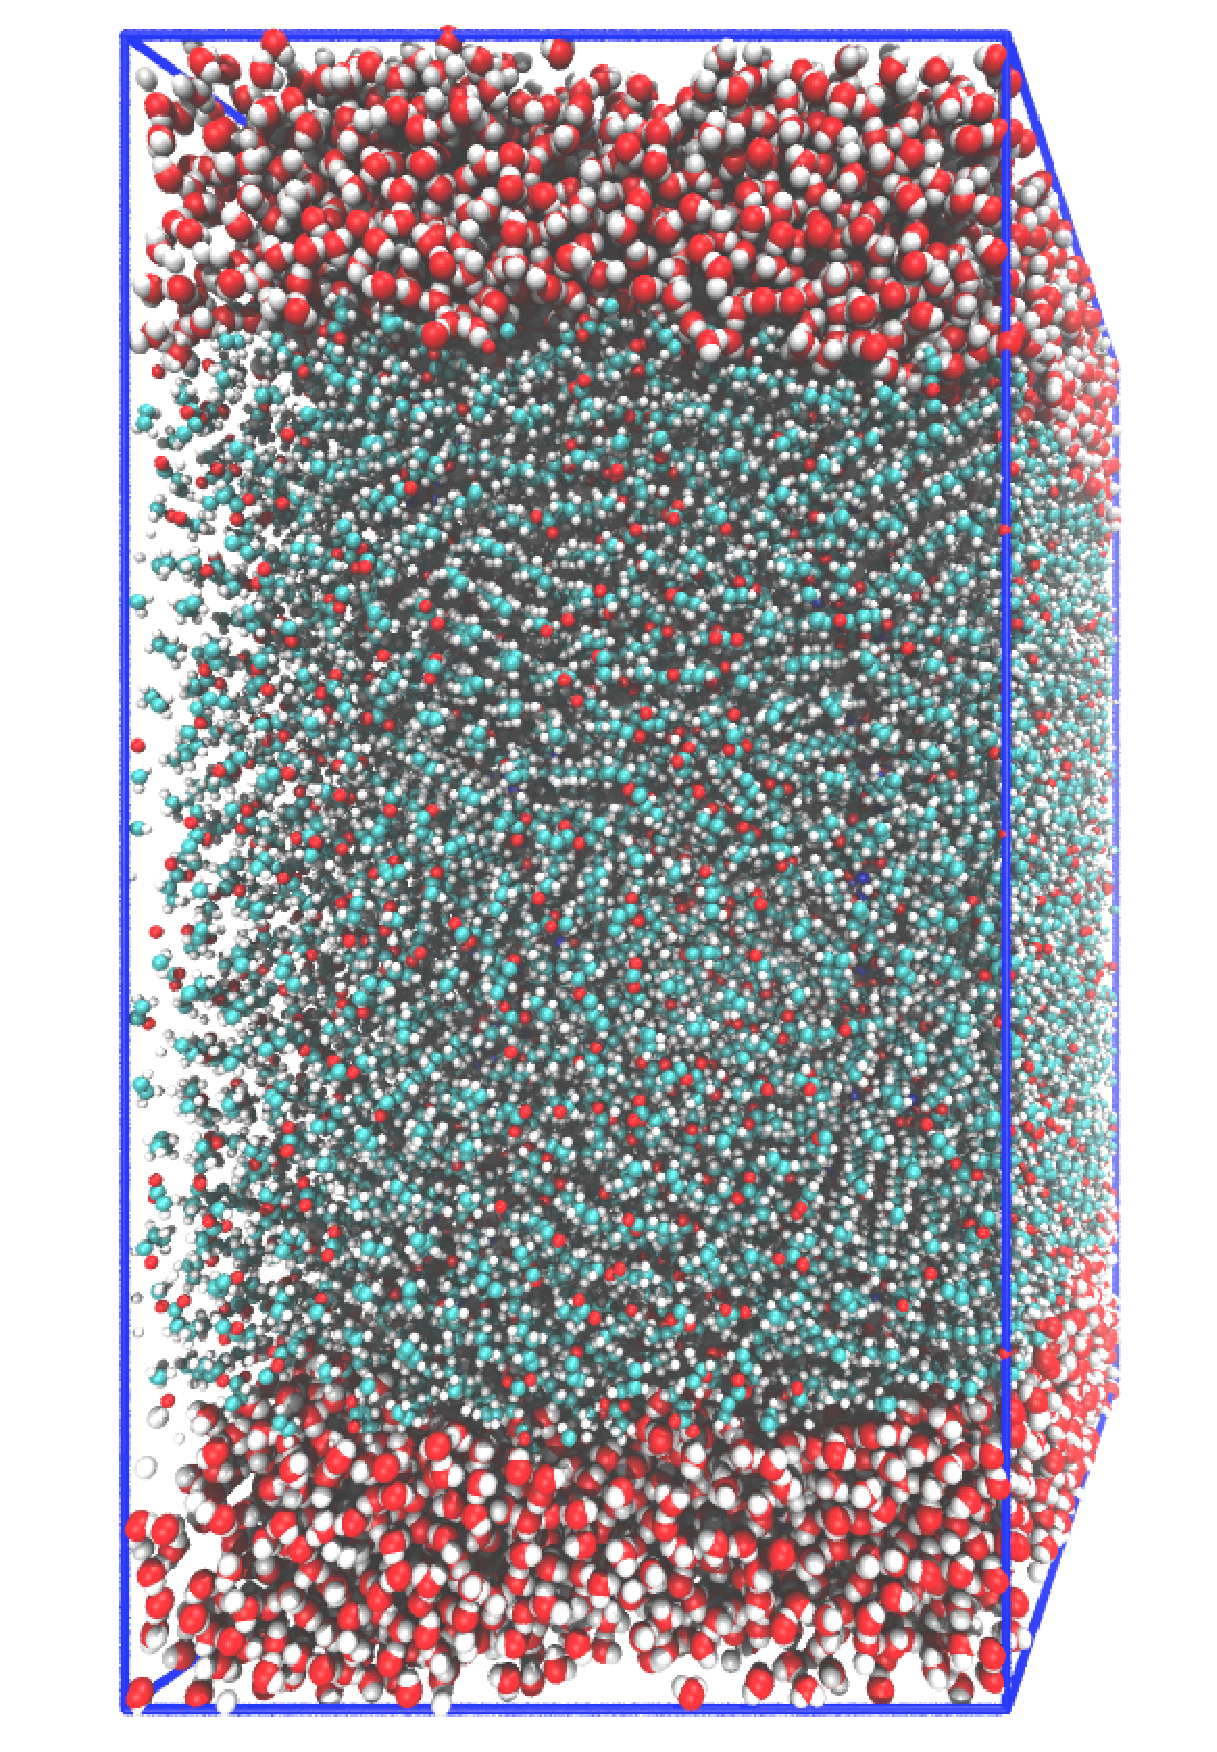
\includegraphics[width=\linewidth]{gap.pdf}
  \caption{}\label{fig:gap}
  \end{subfigure}  
  \begin{subfigure}{0.37\textwidth}
% Generated with : solute_partitioning.py -t shifted.xtc -g berendsen.gro -buffer 2 -r SOL
% in directory : /home/bcoscia/Documents/Gromacs/equilibration/solvation_equilibration/NaGA3C11/gaps/pre_equilibrated
  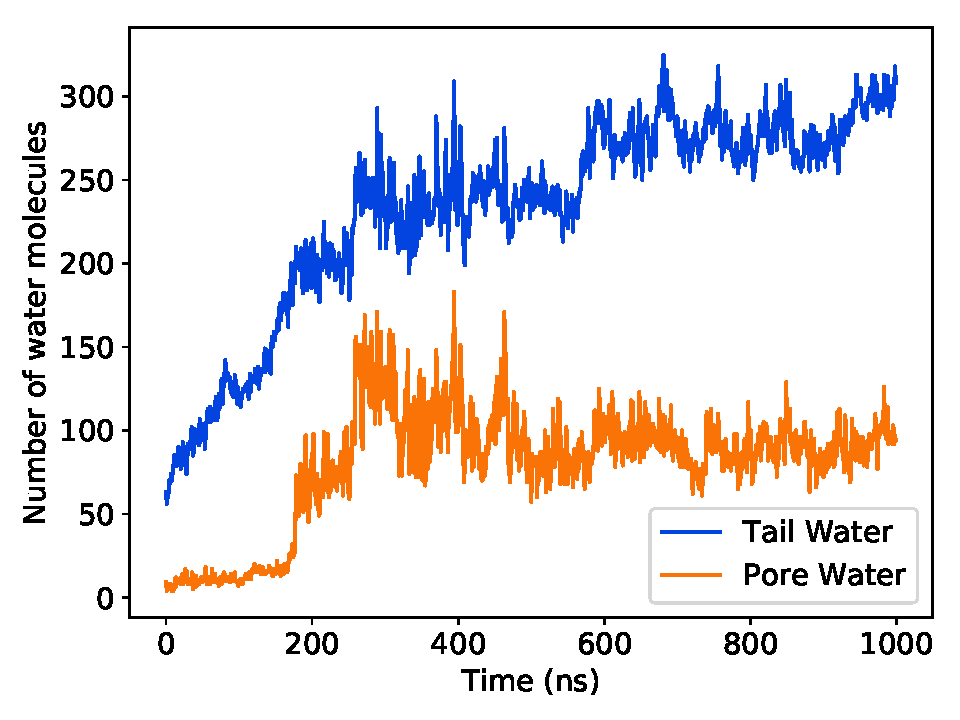
\includegraphics[width=\linewidth]{equilibrated_water_penetration.pdf}
  \caption{}\label{fig:equilibrated_water_penetration}
  \end{subfigure}  
  \begin{subfigure}{0.37\textwidth}
% Generated with custom script density.py located in same directory as above.
  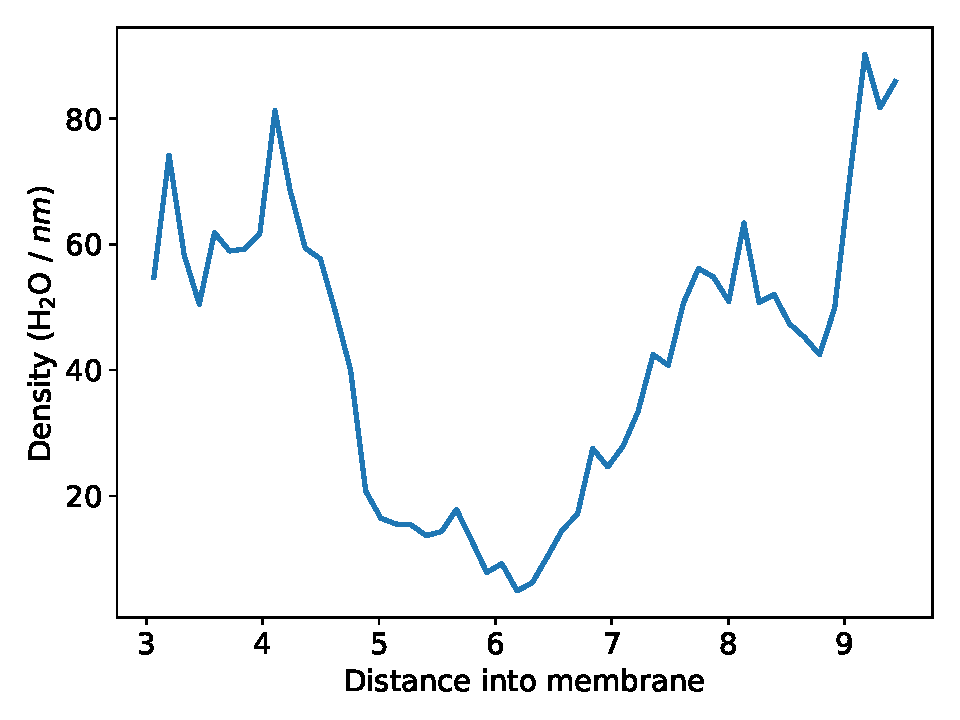
\includegraphics[width=\linewidth]{penetration_density.pdf}
  \caption{}\label{fig:penetration_density}
  \end{subfigure}  
  \caption{(a) Using an equilibrated dry configuration, we inserted a 3 nm thick layer 
  of water between periodic copies of the system in the $z$-direction. (b) Water slowly
  enters the membrane. Most water enters the tail region where the density of monomers
  is lowest. Water entering the pore plateaus after 500 ns. (c) Although the water
  content of the pore appears equilibrated in (b), the density of water throughout
  the pores is not uniform, with almost no water close to the pore center. Note that
  the density is not shown below 3 nm or above 9.5 nm, because the the system
  enters the water layer at those points.
  }\label{fig:gap_solvation}
  \end{figure}

  We equilibrated 4 systems where we initially placed water in the pores and in
  the tails in addition to a water reservoir between periodic images. We filled
  the pores with water by running \texttt{gmx solvate} on our initial
  configuration and removing any water molecules placed in the tail region. The
  GROMACS command \texttt{gmx solvate} places water molecules in proximity to
  other atoms based on their van der Waals radii and therefore does
  a decent job of preventing equilibration issues. This also means that the
  initial pore radius dictates the water content of the pore. We can however, put
  arbitrary amounts of water into the tail region. We chose to test systems with
  initial pore radii of 5, 6, 7 and 8 \AA~with tail and pore water compositions
  given in Table~\ref{table:water_content}.

  \begin{table}[!htb]
  \centering
  \begin{tabular}{|c|c|c|}
  \hline
  Pore Radius (\AA) & wt \% water tails & wt \% water pores \\
  \hline
  5                 &        5.67       &     1.09          \\
  6                 &        2.88       &     2.38          \\
  7                 &        1.91       &     4.12          \\
  8                 &        2.78       &     6.00          \\
  \hline
  \end{tabular}
  \caption{We chose a diverse combination of initial pore and tail water
  contents in order to study its effect on equilibrium water
  content.}\label{table:water_content}
  \end{table}

  Systems appear to be most stable when there is more water in the pores than
  tails. In systems started with more water in the tails
  (Figures~\ref{fig:r5_gap} and \ref{fig:r6_gap}), the pore water content tends
  to increase over time, while that of the tails decreases or stays stable.
  Filling the pores with water is likely a very long process since it requires
  monomers to make space for water molecules. Systems started with a higher pore
  water content (Figures~\ref{fig:r7_gap} and \ref{fig:r8_gap}) tend to plateau
  relatively quickly, with about one third of the water staying in the tails.  We
  used this ratio in order to construct the initial configurations used for the
  studies in the main text.  Clearly, a more complicated methodology is needed in
  order to predict the equilibrium water content of a given LLC membrane.
  However, getting the value exactly right is not required for our study.
  Instead, we can observe mechanisms as a function of water content in each
  region. 

  \begin{figure}[!htb]
  \centering
  \begin{subfigure}{0.45\textwidth}
% Generated by running: solute_partitioning.py -t stabilized.xtc -g PR.gro -buffer 3 --savename water_partition.pl
% In directory: /home/bcoscia/Documents/Gromacs/equilibration/solvation_equilibration/NaGA3C11/water_content_experiments/5/1.09_5.67
  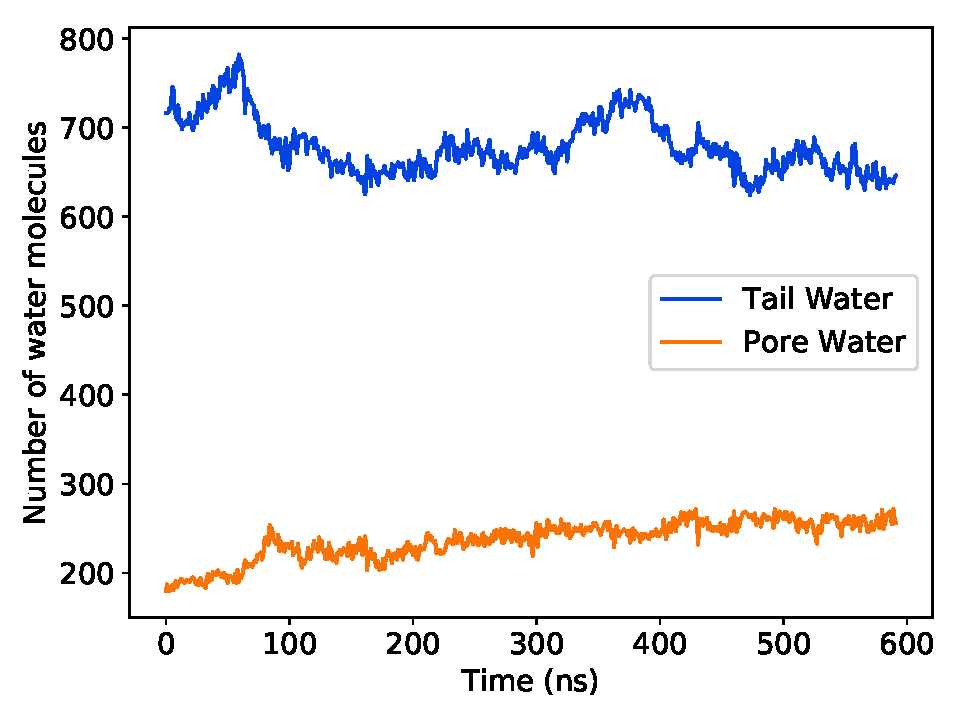
\includegraphics[width=\linewidth]{r5_gap.pdf}
  \caption{r = 5~\AA}\label{fig:r5_gap}
  \end{subfigure}
  \begin{subfigure}{0.45\textwidth}
% Generate by running: solute_partitioning.py -t stabilized.xtc -g PR.gro -buffer 2.5 -r SOL --savename water_partition.pl
% In directory: /home/bcoscia/Documents/Gromacs/equilibration/solvation_equilibration/NaGA3C11/water_content_experiments/6/2.38_2.88
  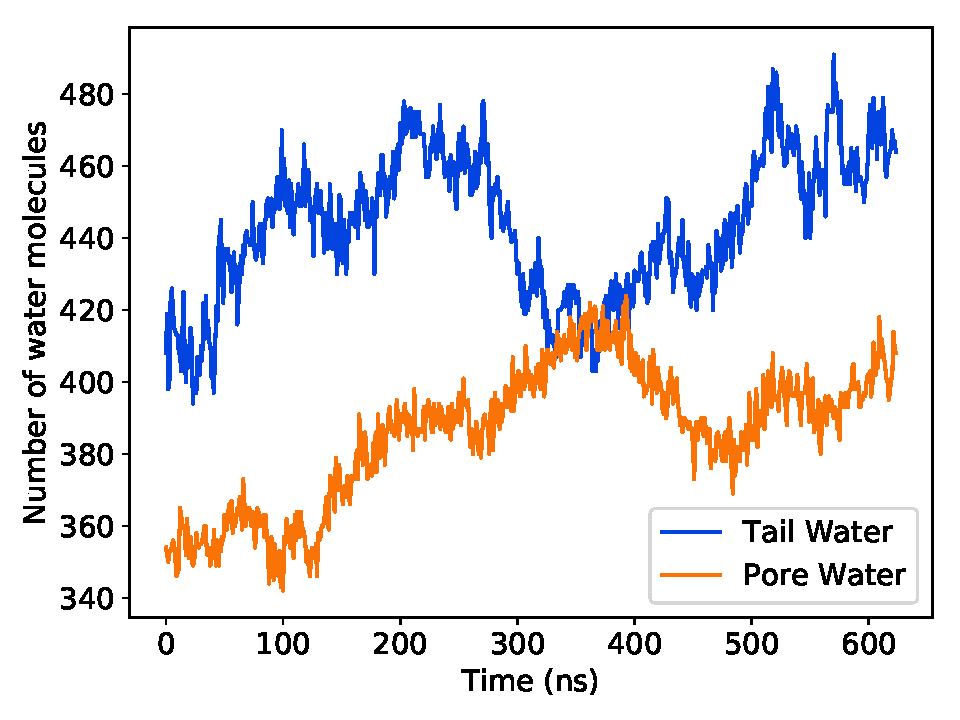
\includegraphics[width=\linewidth]{r6_gap.pdf}
  \caption{r = 6~\AA}\label{fig:r6_gap}
  \end{subfigure}
  \begin{subfigure}{0.45\textwidth}
% Generate by running: solute_partitioning.py -t stabilized.xtc -g last.gro -buffer 3 -r SOL --savename water_partition.pl
% In directory: /home/bcoscia/Documents/Gromacs/equilibration/solvation_equilibration/NaGA3C11/water_content_experiments/6/4.12_1.91
  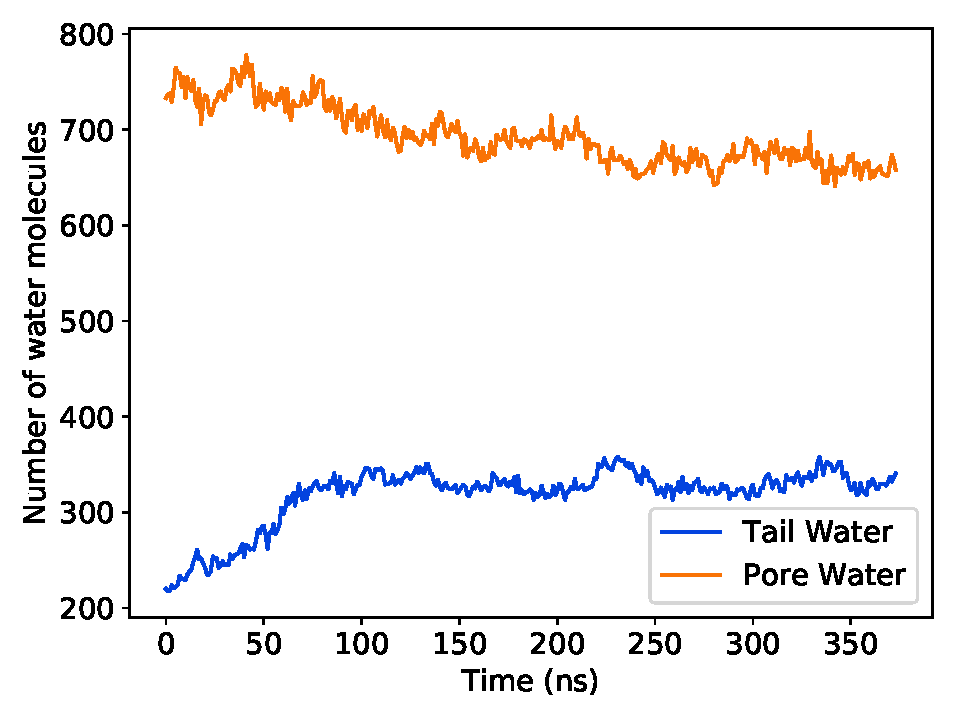
\includegraphics[width=\linewidth]{r7_gap.pdf}
  \caption{r = 7~\AA}\label{fig:r7_gap}
  \end{subfigure}
  \begin{subfigure}{0.45\textwidth}
% Generate by running: solute_partitioning.py -t stabilized.xtc -g last.gro -buffer 3 -r SOL --savename water_partition.pl
% In directory: /home/bcoscia/Documents/Gromacs/equilibration/solvation_equilibration/NaGA3C11/water_content_experiments/8/6.00_2.78
  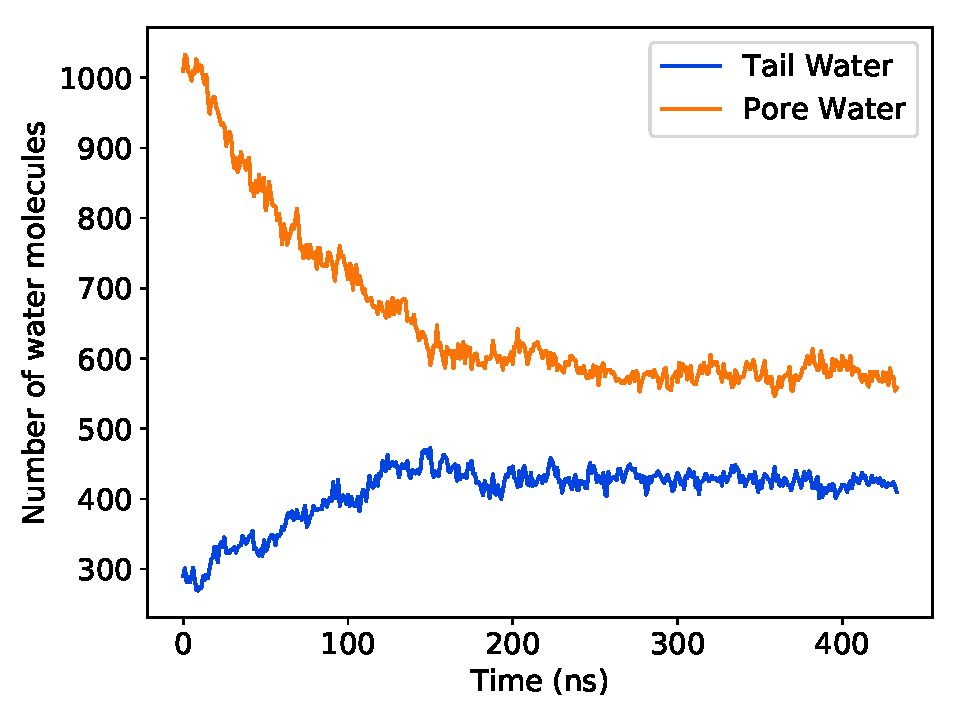
\includegraphics[width=\linewidth]{r8_gap.pdf}
  \caption{r = 8~\AA}\label{fig:r8_gap}
  \end{subfigure}
  \caption{There is likely more water in the pore region than in the tail region.
  When we create configurations with more water in the tails, equilibration is 
  slow. When configurations start with more water in the pores, the water content
  in each region equilibrates quickly.}\label{fig:gap_prefilled_equil}
  \end{figure}

  Since the equilibrium water content is unclear based on the previous
  simulations, we elected to choose and study systems with two different water
  contents. We removed the water reservoir and allowed the pore and tail water
  contents to equilibrate with 5 and 10 wt \% total water. We placed one third of
  the total water needed in the tails, based on the intuition gained in
  Figure~\ref{fig:gap_prefilled_equil}. We considered the water content
  equilibrated once the water contents plateaued. The 5 wt\% system did
  not plateau until $\sim$ 600 ns (Figure~\ref{fig:5wt_offset_equil})
  while the 10 wt \% water system equilibrated within the first 100 ns of 
  simulation (Figure~\ref{fig:10wt_offset_equil}).
  The pores contain 72 \% and 69 \% of the total water in the 5 and 10 wt \%
  systems respectively.

  \begin{figure}[!htb]
  \centering
  \begin{subfigure}{0.45\textwidth}
% Generated with solute_partitioning.py -t full_shifted.xtc -g berendsen.gro -r SOL -pr 1.6 --savename water_partitioning.pl
% in directory /home/bcoscia/Documents/Gromacs/equilibration/solvation_equilibration/NaGA3C11/offset/5wt
  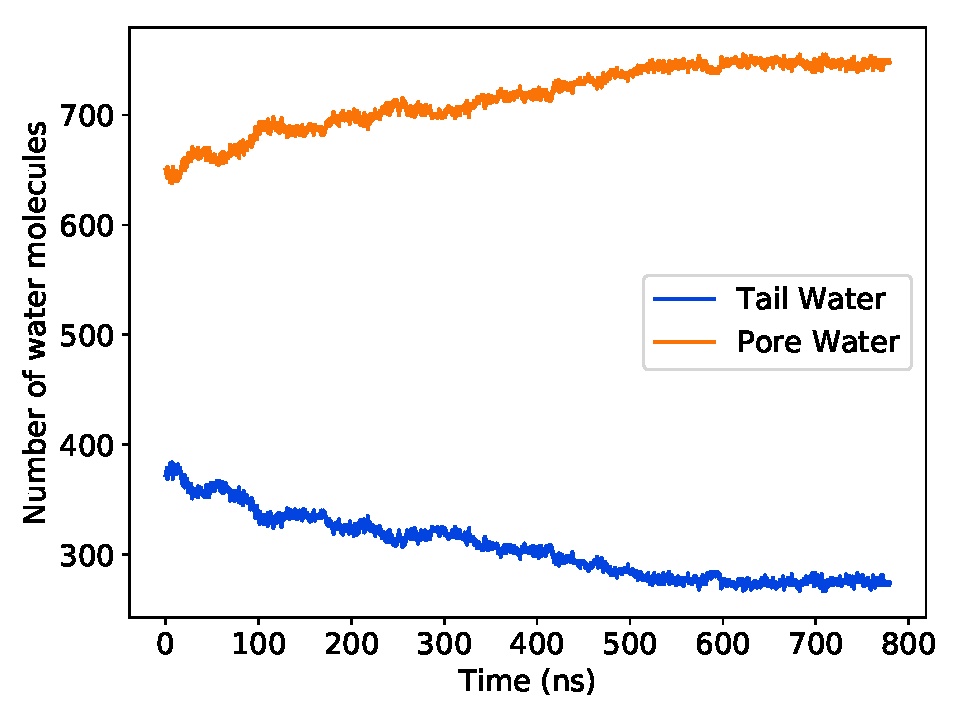
\includegraphics[width=\textwidth]{5wt_offset_equil.pdf}
  \caption{5 wt \%}\label{fig:5wt_offset_equil}
  \end{subfigure}
  \begin{subfigure}{0.45\textwidth}
  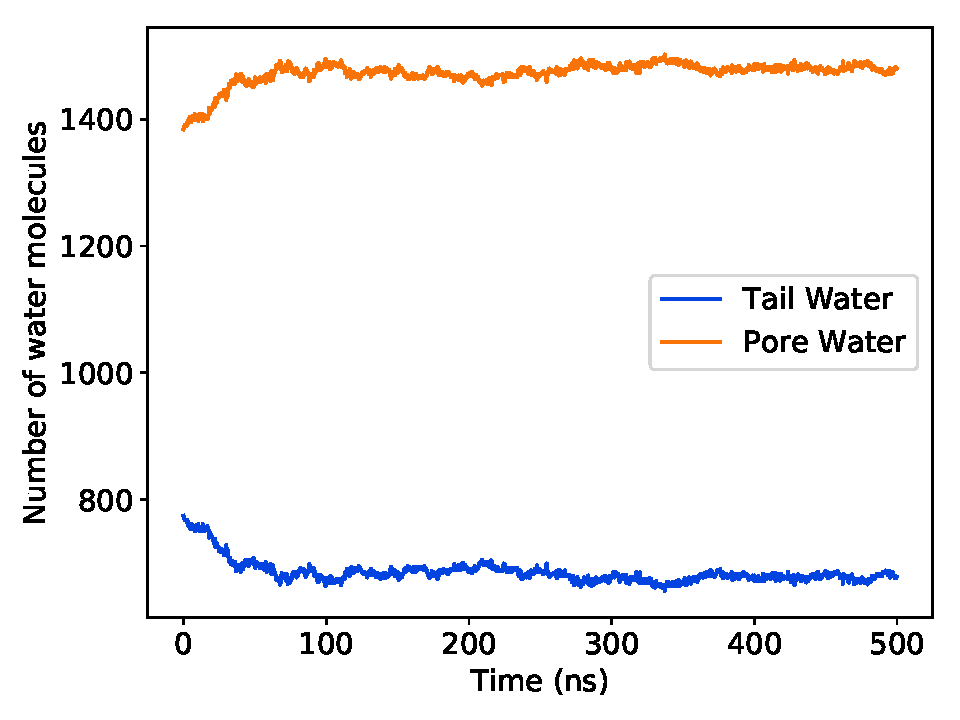
\includegraphics[width=\textwidth]{10wt_offset_equil.pdf}
  \caption{10 wt \%}\label{fig:10wt_offset_equil}
% Generated with solute_partitioning.py -t shifted.xtc -g last.gro -r SOL -pr 1.48 --savename water_partitioning.pl
% in directory /home/bcoscia/Documents/Gromacs/equilibration/solvation_equilibration/NaGA3C11/offset/10wt
  \end{subfigure}
  \caption{We created solvated systems with one third of the total water
	  initially placed in the tail region. (a) With 5 wt \% total water, the water
	  content equilibrates after 600 ns, with $\sim$ 72 \% of the total water in the
	  pores. (b) With 10 wt \% total water, the water content equilibrates after 100
	  ns, with $\sim$ 69 \% of the total water in the
	  pores.}\label{fig:solvation_equilibration}
  \end{figure}

  We cross-linked the equilibrated solvated systems, then allowed them to 
  equilibrate further for 100 ns. The water contents in each region does not
  change significantly in either case.

  \begin{figure}[!htb]
  \centering
  \begin{subfigure}{0.45\textwidth}
% Generated with solute_partitioning.py -t PR.trr -g PR.gro -r SOL --savename SOL_partitioning.pl
% In directory /home/bcoscia/Documents/Gromacs/equilibration/xlink_equilibration/NaGA3C11/5wt
  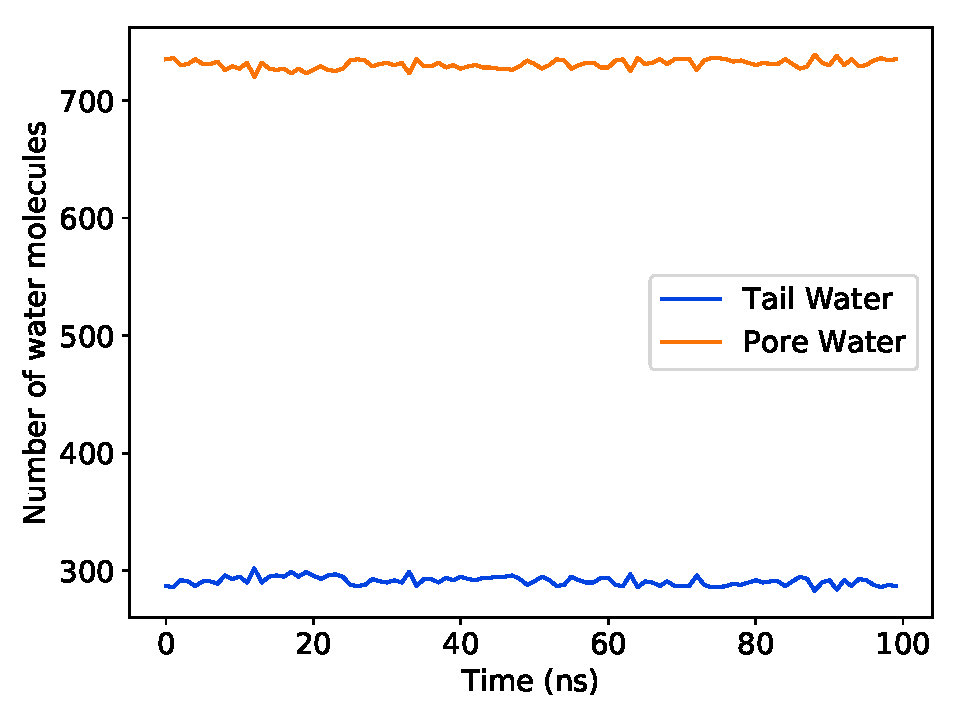
\includegraphics[width=\textwidth]{5wt_offset_xlinked_equil.pdf}
  \caption{5 wt\%}\label{fig:5wt_offset_xlinked_equil}
  \end{subfigure}
  \begin{subfigure}{0.45\textwidth}
  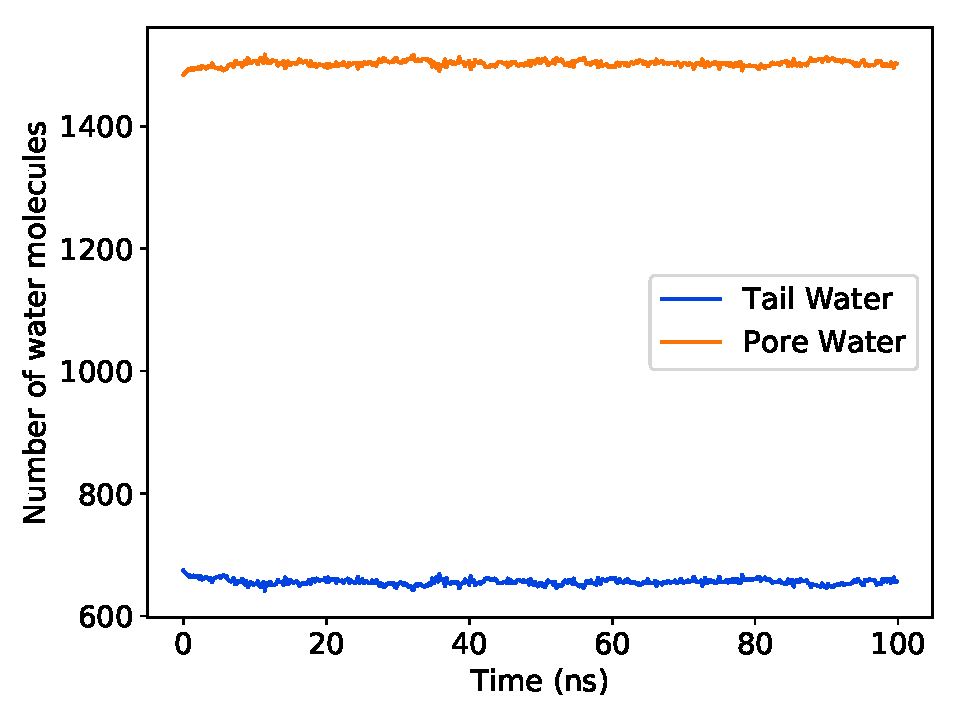
\includegraphics[width=\textwidth]{10wt_offset_xlinked_equil.pdf}
  \caption{10 wt\%}\label{fig:10wt_offset_xlinked_equil}
% Generated with solute_partitioning.py -t xlinked_equil.trr -g xlinked_equil.gro -r SOL -pr 1.48 --savename water_partitioning.pl
% In directory /home/bcoscia/Documents/Gromacs/equilibration/xlink_equilibration/NaGA3C11/10wt/63_percent
  \end{subfigure}
  \caption{The water content in the tail and pore region is not affected
  by cross-linking}\label{fig:solvation_equilibration}
  \end{figure}  
  
  \clearpage  
  
  \section{Solute Interaction}\label{section:solute_interaction}
  
  We chose to model 6 solutes in each pore because there was a low degree of 
  interaction between solutes which gave us a sufficient number of independent 
  trajectories to observe and analyze. There are a negligible number of occurrences
  % BJC: not sure what the appropriate cut-off should be
  where the center of a given solute came within 3.5 \AA~of another same-solute
  center of mass.
  
  \begin{figure}[!htb]
  \centering
  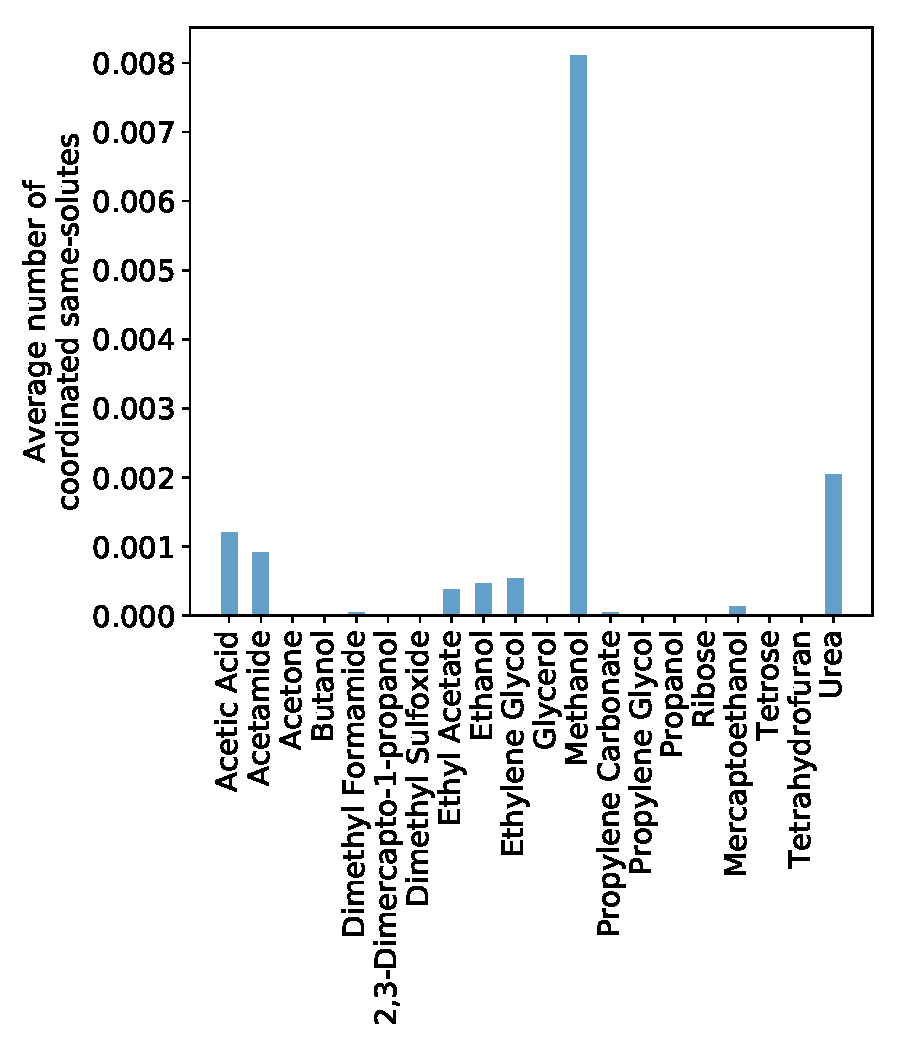
\includegraphics[width=0.45\textwidth]{solute_interaction.pdf}
  \caption{Interactions between same-solutes are negligible when systems are 
  built with 6 solutes per pore. Even methanol, which interacts with other same-solute
  molecules the most, does so less than 0.05 \% of the time.}\label{fig:solute_interaction}
  \end{figure}
  
%  \subsection{Sensitivity of Breakdown radius of Stokes-Einstein Equation}\label{section:se_sensitivity}
%  
%  In the main text, we estimated the trend in solute MSDs using the Stokes-Einstein
%  equation with the correction factor of Gierer and Wirtz, $f$, given by 
%  equation~\ref{M-eqn:correction_factor}. As $r \rightarrow \infty$ , $f \rightarrow 1$.
%  
%  We assumed that the Stokes-Einstein relationship could be approximated as a
%  piecewise function where the correction factor of Gierer and Wirtz, $f$, given
%  by equation~\ref{M-eqn:correction_factor} of the main text, is only applied below
%  a critical radius. At radii greater than the critical radius, $f$ = 1.
%  
%  In the main text, we constrained the corrected Stokes-Einstein equation so that
%  it passed through the highest MSD value. We also plotted the uncorrected 
%  Stokes-Einstein equation ($f$=1) as a lower bound to our expectations for 
%  unrestricted solute motion. The lower bound is relatively insensitive to our
%  choice of critical radius. Even for an unrealistically small critical radius 
%  of 0.5 nm, the curve is within
%  
%  \begin{figure}[!htb]
%  \centering
%  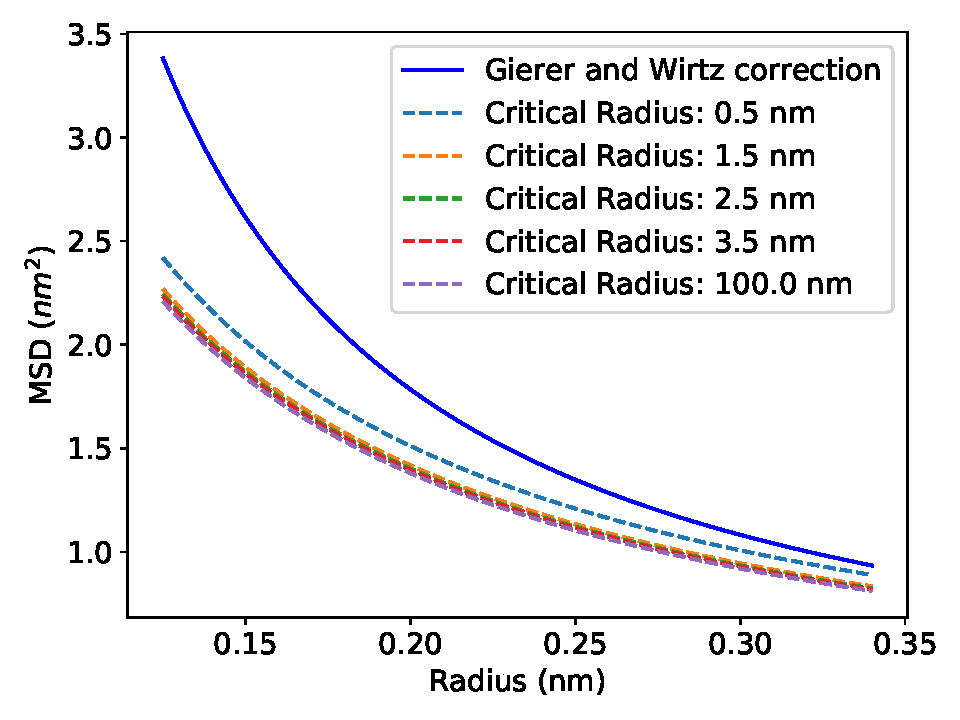
\includegraphics[width=0.45\textwidth]{stokes_intersection_sensitivity.pdf}
%  \caption{We varied the molecular radius at which we assumed the Stokes-Einstein
%  (SE) relationship to breaks down. It is assumed that the Gierer and Wirtz correction
%  to the SE equation becomes a more accurate estimation of MSD at small radii, after
%  the point of intersection }\label{fig:se_intersection_sensitivity}
%  \end{figure}
  \clearpage
  \section{Solute MSD Ranking Time Lag Sensitivity}\label{section:lag_sensitivity}
  
  We chose to report the MSD of our solutes after a 400 ns time lag. This choice does
  not have a significant influence on the ranking of the solute MSDs. Although there
  is minor re-ranking among solutes with similar MSDs, it does not affect any of 
  the conclusions drawn in the main text.
  
  \begin{figure}[!htb]
  \centering
  \begin{subfigure}{0.325\textwidth}
  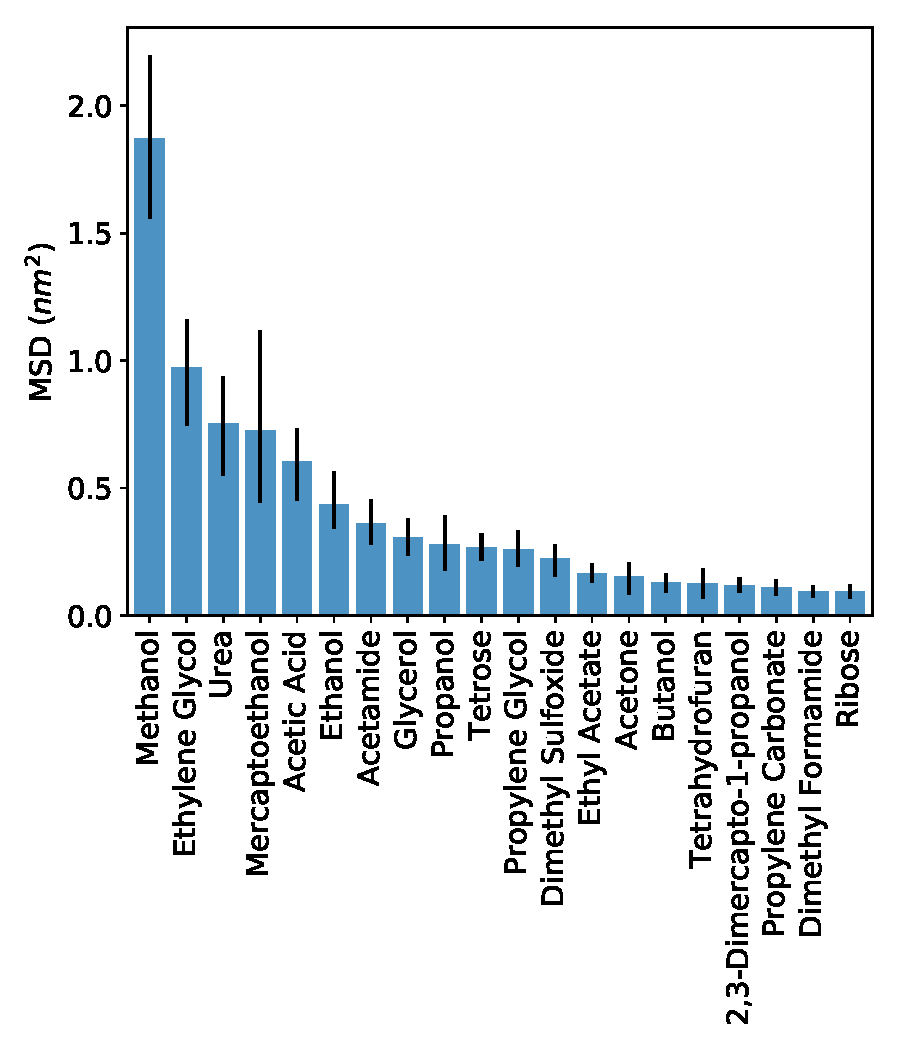
\includegraphics[width=\textwidth]{all_10wt_tamsds_F0_2.pdf}
  \caption{Time lag = 200 ns}\label{fig:F0.2}
  \end{subfigure}
  \begin{subfigure}{0.325\textwidth}
  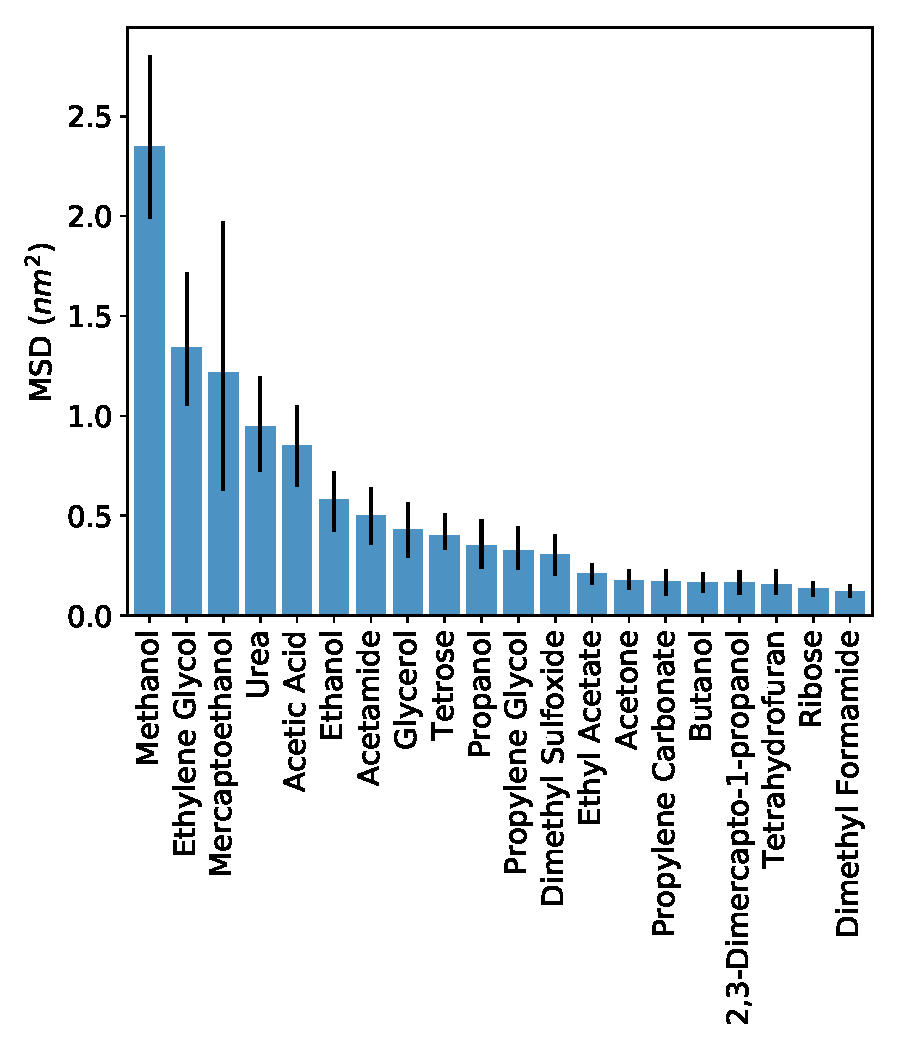
\includegraphics[width=\textwidth]{all_10wt_tamsds_F0_3.pdf}
  \caption{Time lag = 300 ns}\label{fig:F0.3}
  \end{subfigure}
  \begin{subfigure}{0.325\textwidth}
  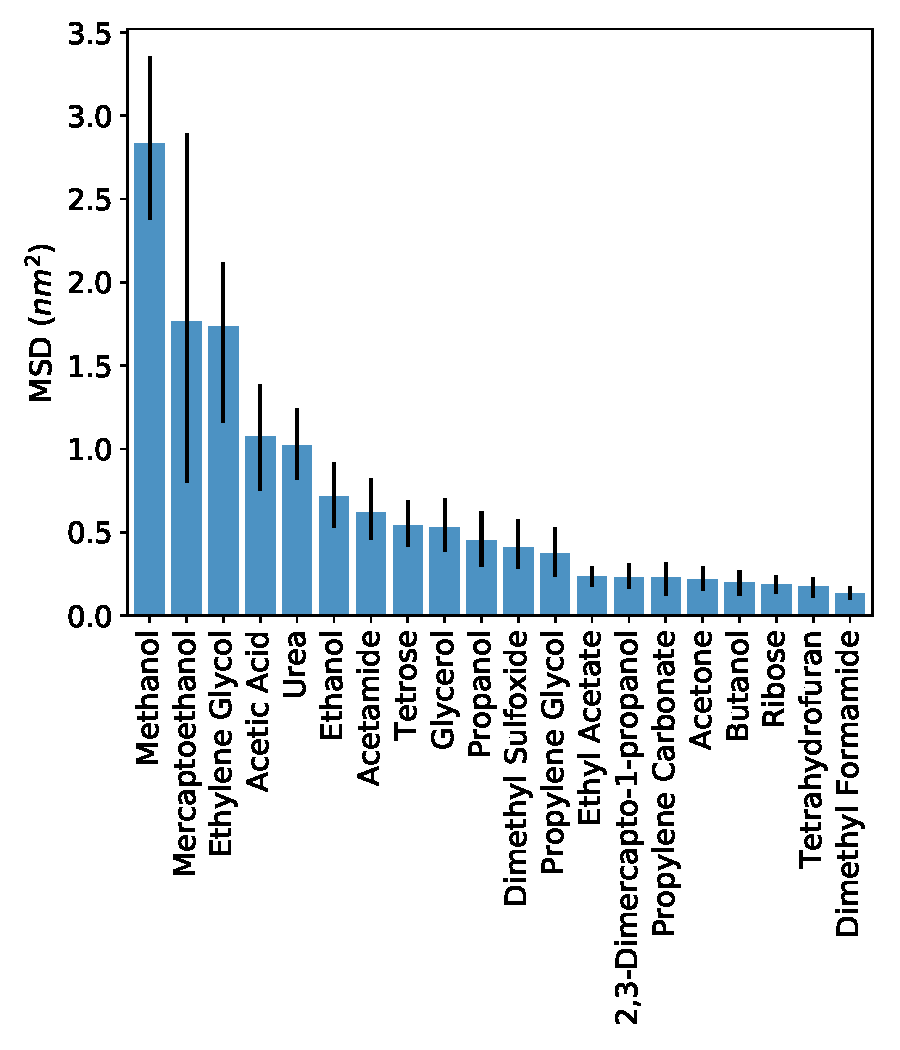
\includegraphics[width=\textwidth]{all_10wt_tamsds_F0_4.pdf}
  \caption{Time lag = 400 ns}\label{fig:F0.4}
  \end{subfigure}
  \begin{subfigure}{0.325\textwidth}
  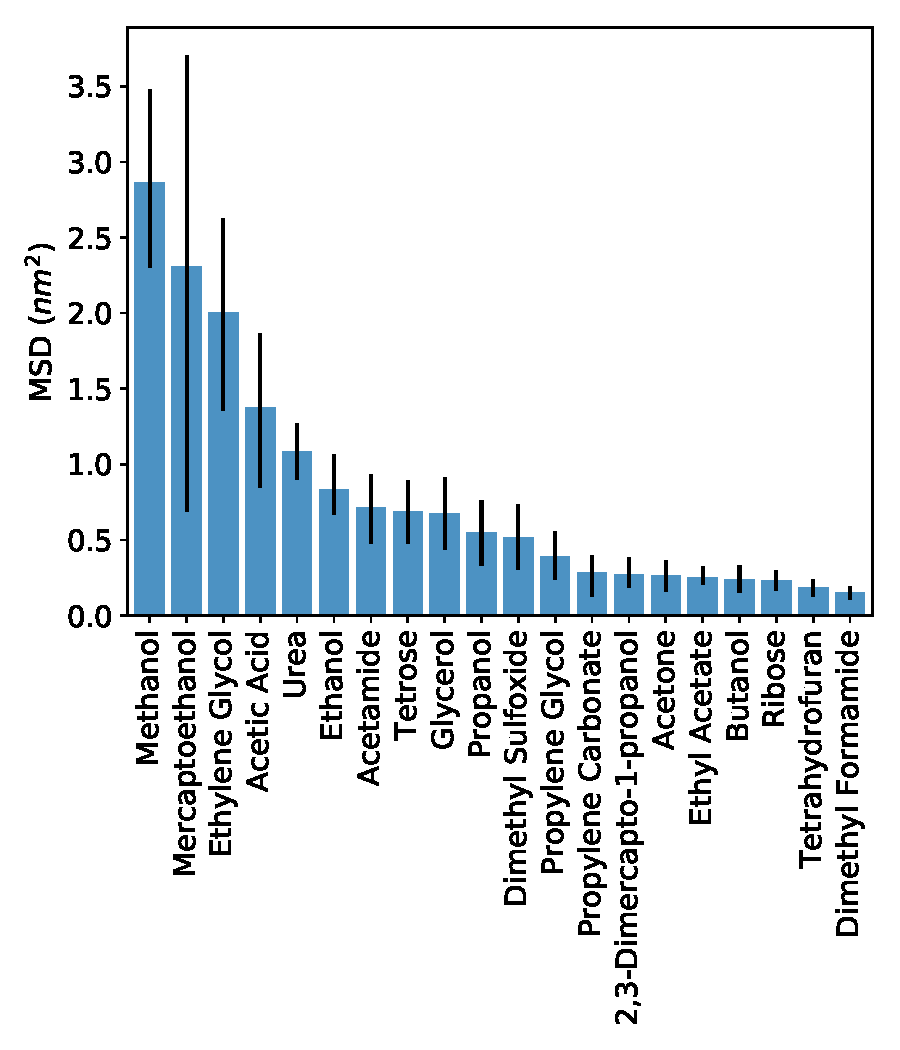
\includegraphics[width=\textwidth]{all_10wt_tamsds_F0_5.pdf}
  \caption{Time lag = 500 ns}\label{fig:F0.5}
  \end{subfigure}
  \begin{subfigure}{0.325\textwidth}
  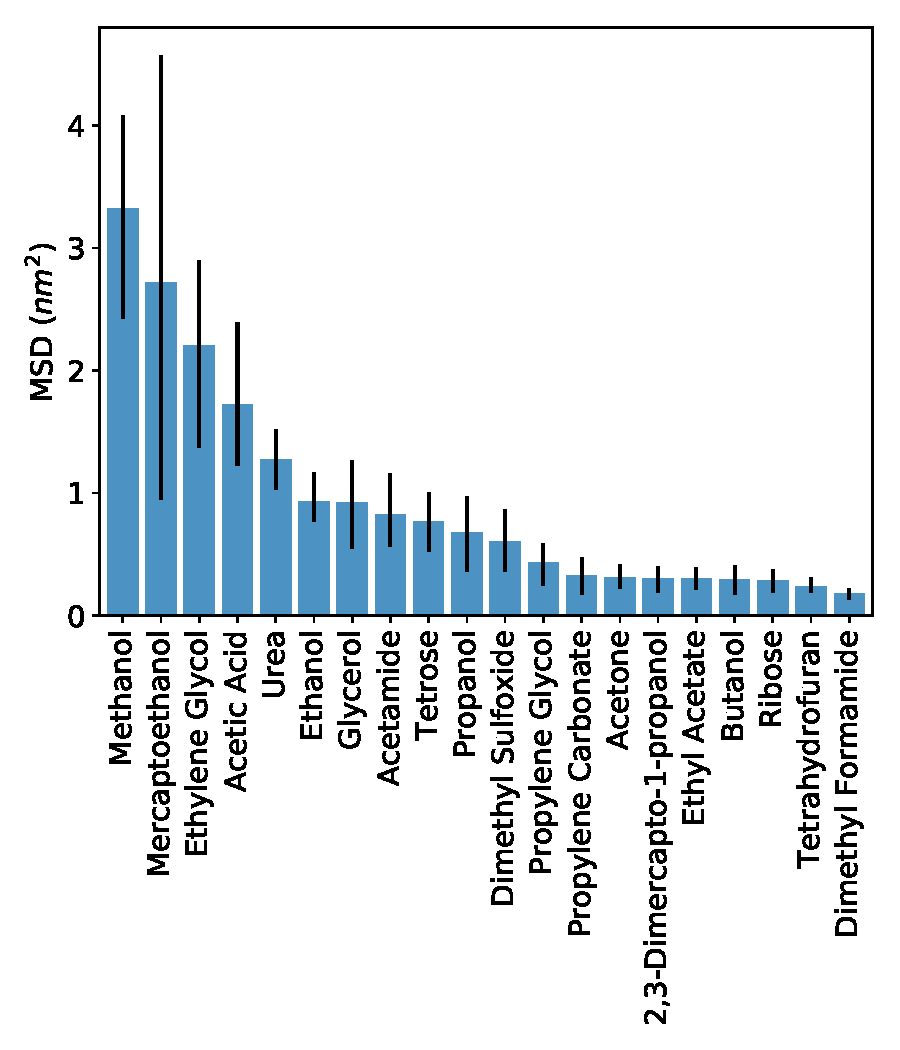
\includegraphics[width=\textwidth]{all_10wt_tamsds_F0_6.pdf}
  \caption{Time lag = 600 ns}\label{fig:F0.6}
  \end{subfigure}
  \caption{The choice of time lag used to report solute MSDs does not 
  influence the trends reported in the main text. We observe minor re-ranking
  of solutes with similar MSDs and note that longer time lags generally
  lead to large error bars on the MSDs, as expected. }\label{fig:lag_sensitivity}
  \end{figure}
  
  \clearpage
  \section{Pore Region Definition}\label{section:pore-region}
  
  We performed a sensitivity analysis in order to determine the radial 
  cut-off that maximizes the difference in hop lengths in and out of 
  the pore region. We varied the location of the cut-off defining the
  edge of the pore region in increments of 0.05 from 0.3 to 0.7. We
  varied the cut-off in increments of 0.01 from 0.7 to 0.8 in order to
  increase our resolution about the maximum (see Figure~\ref{fig:pore_cutoff}). 
  Defining the cut-off 0.75 nm from the pore center maximizes the 
  difference in hop lengths between solutes in and out of the pore.
  
  \begin{figure}
  \centering
  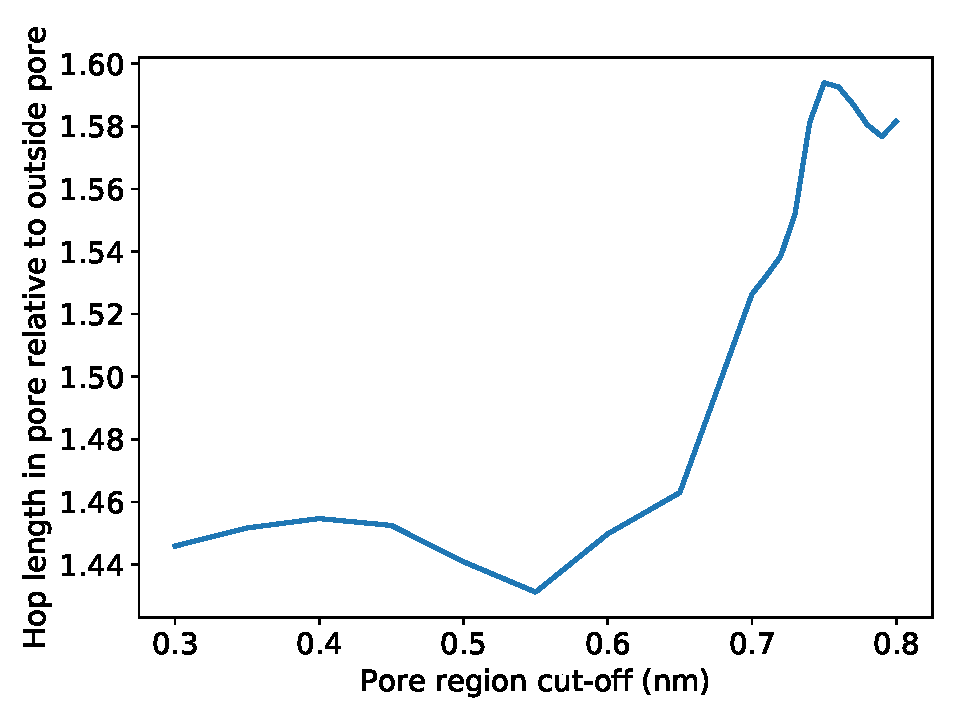
\includegraphics[width=0.5\linewidth]{pore_cutoff.pdf}
  \caption{Defining the cut-off 0.75 nm from the pore center maximizes the 
  difference in hop lengths between solutes in and out of the pore. We 
  varied the location of the cut-off defining the edge of the pore region
  in increments of 0.05 from 0.3 to 0.7. We varied the cut-off in 
  increments of 0.01 from 0.7 to 0.8 in order to increase our resolution
  about the maximum.}\label{fig:pore_cutoff}
  \end{figure}

  \clearpage
  \section{Hydrogen Bond Detection Sensitivity}\label{section:hbond_sensitivity}
  
  In Section 2.8 of the main text, we established geometric criteria for the 
  identification of hydrogen bond interactions. Namely, if the distance between the donor,
  D, and acceptor, A, atoms is less than 3.5 \AA~and the angle formed by D--H...A is less
  than 30\degree, then we consider the interaction to be a consequence of hydrogen bonding.
  
  \begin{figure}[!htb]
  \centering
  \begin{subfigure}{\textwidth}
  \centering
  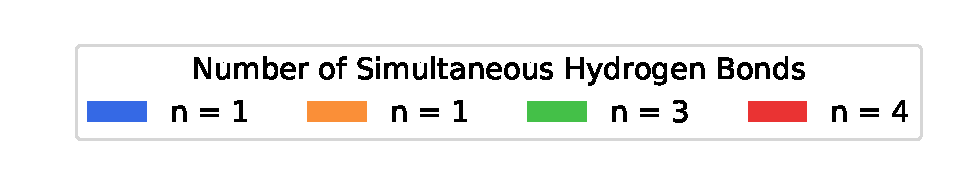
\includegraphics[trim={0 0.5cm 0.5cm 0.5cm}, clip, width=0.5\textwidth]{hbond_sensitivity_legend.pdf}
  \end{subfigure}
  \begin{subfigure}{\textwidth}
  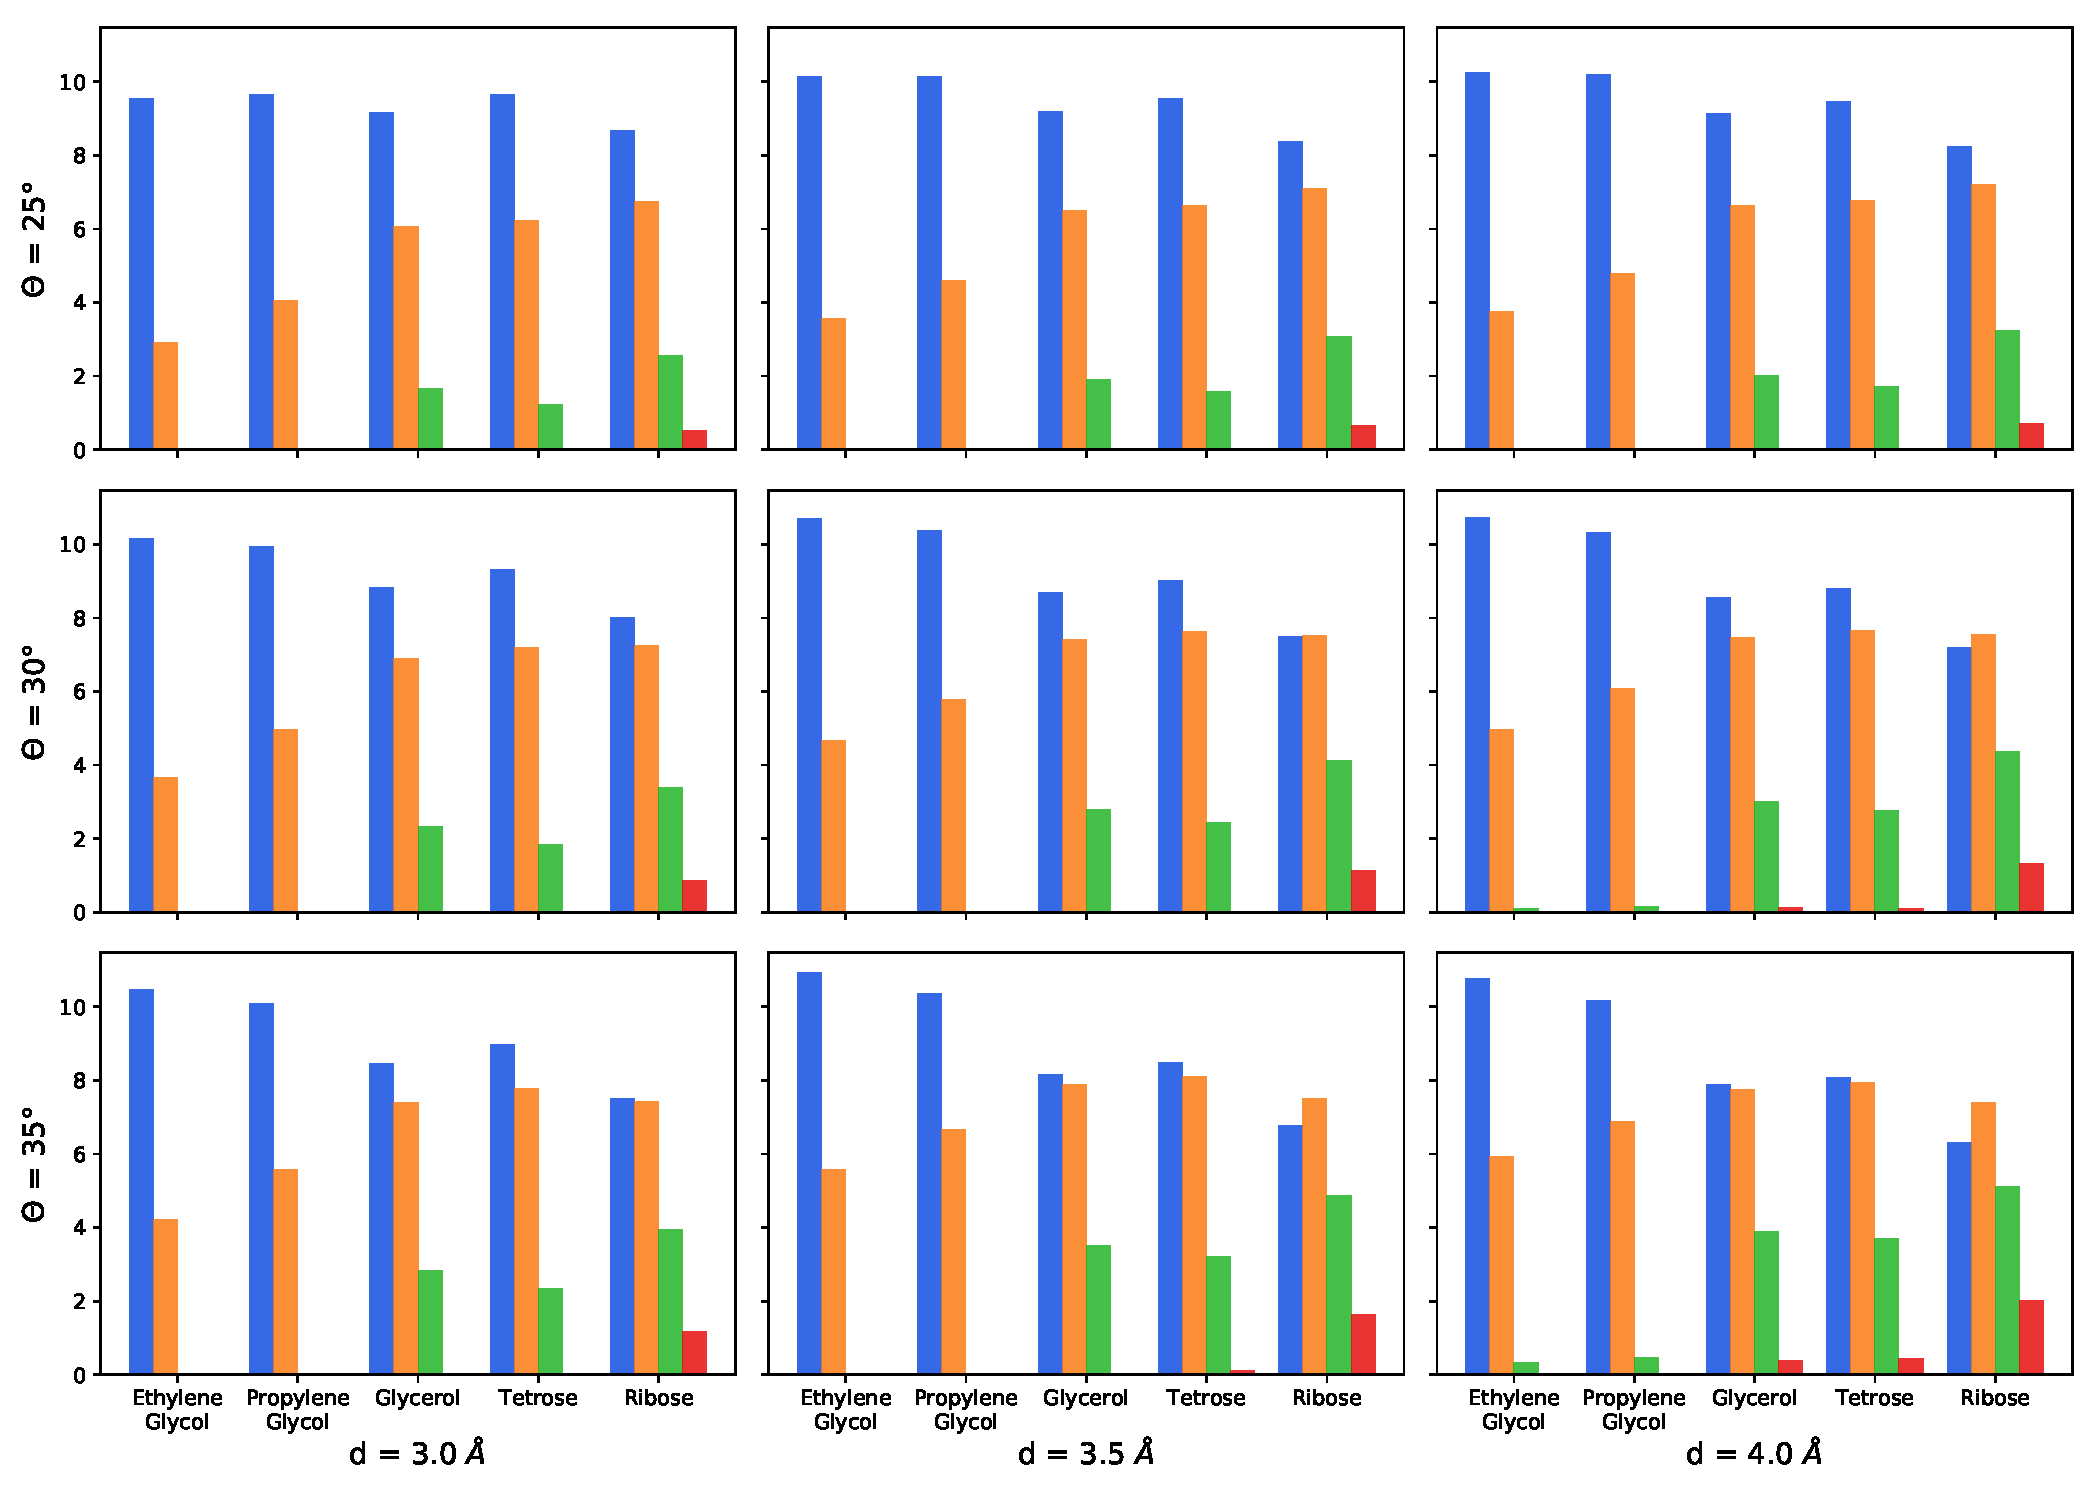
\includegraphics[width=\textwidth]{hbond_sensitivity.pdf}
  \end{subfigure}
  \caption{We tested the sensitivity of our hydrogen bond detection to the chosen 
  geometric criteria for hydrogen bonding. We varied the distance cut-off between 3.0 and
  4.0 \AA, and varied the angle cut-off between 25 and 35 \degree.}\label{fig:hbond_sensitivity}
  \end{figure}
  
  We tested the sensitivity of this criteria to ensure that our conclusions
  were not a strong function of the chosen criteria. In Figure~\ref{fig:hbond_sensitivity} we
  plotted the results of the same calculation performed to create Figure~\ref{M-fig:multi_hbonds}c
  of the main text. We varied the distance cut-off between 3.0 and 4.0 \AA, and varied the
  angle cut-off between 25 and 35 \degree. 
  
  As the distance and angle cut-offs are increased, there is a slight increase in the total
  number of hydrogen bonds, which is primarily manifested by an increased number of multiple-hydrogen-bond
  interactions. Using our most lenient set of criteria (d = 4.0 \AA~and $\theta$ = 35 $\degree$), glycerol,
  tetrose and ribose all show instances where they simultaneously hydrogen bond with 4 head group atoms.
  In the strictest case (d = 3.0 \AA~and $\theta$ = 25 \degree), ribose is the only solute with a 
  detected instance of a quadruple hydrogen bond.
  
  We can draw the same conclusions from any of the plots in Figure~\ref{fig:hbond_sensitivity}:
  \begin{enumerate}
    \item An increased number of hydroxyl groups results in an increased number of hydrogen bond
    interactions.
    \item The number of multiple-hydrogen-bond interactions increases.
    \item On average, propylene glcyol participates in more hydrogen bond interactions than 
    ethylene glycol.  %BJC: might need to label the total hydrogen bonds (put number centered on top of bars)
  \end{enumerate}
  
  \section{Lifetime Distributions}\label{section:lifetime_distributions}
  
  The distribution of hydrogen bond lifetimes and association lifetimes
  for all solutes appears to be power law or exponentially distributed. 
  Example distributions generated from ethylene glycol are shown in
  Figure~\ref{fig:lifetime_distributions}. 
  
  \begin{figure}[!htb]
  \centering
  \begin{subfigure}{0.45\textwidth}
  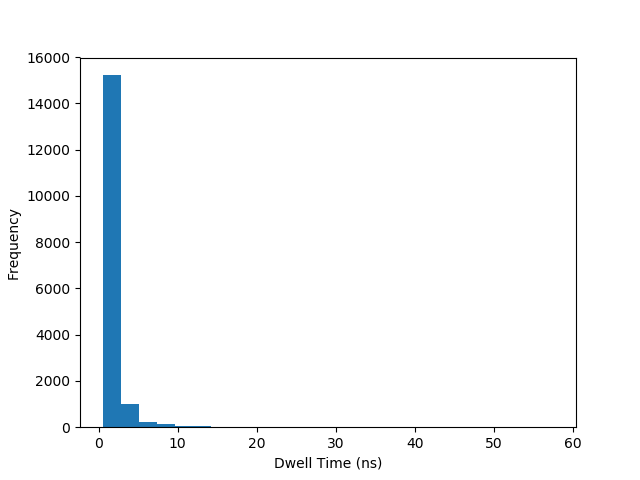
\includegraphics[width=\linewidth]{gcl_hbond_dist.png}
  \caption{}
  \end{subfigure}
  \begin{subfigure}{0.45\textwidth}
  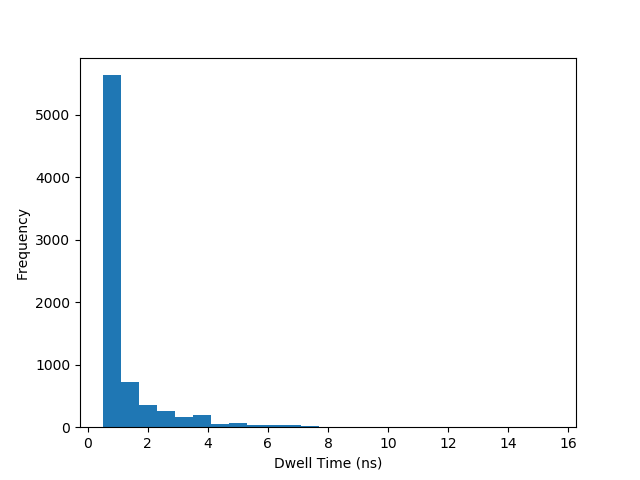
\includegraphics[width=\linewidth]{gcl_coord_dist.png}
  \caption{}
  \end{subfigure}
  \caption{The distribution of hydrogen bond lifetimes and association lifetimes of
  ethylene glycol both appear to be power law or exponentially distributed. We
  do not attempt to distinguish between the type of distribution and instead report
  the 95\% confidence interval of association lifetimes.}\label{fig:lifetime_distributions}
  \end{figure}  
  
  \clearpage
  \section{Pore Splines}\label{section:splines}
  
  We captured the apparent $z$-dependence of the pore center locations by
  constructing splines running through each pore (See Figure~\ref{fig:spline}).
  Each spline consists of 10 points, equally spaced in the $z$-direction, whose
  ($x$, $y$) coordinates are defined based on the center of mass of all head
  groups closest, in $z$, to the given point.
  
  \begin{figure}[!htb]
  \centering
  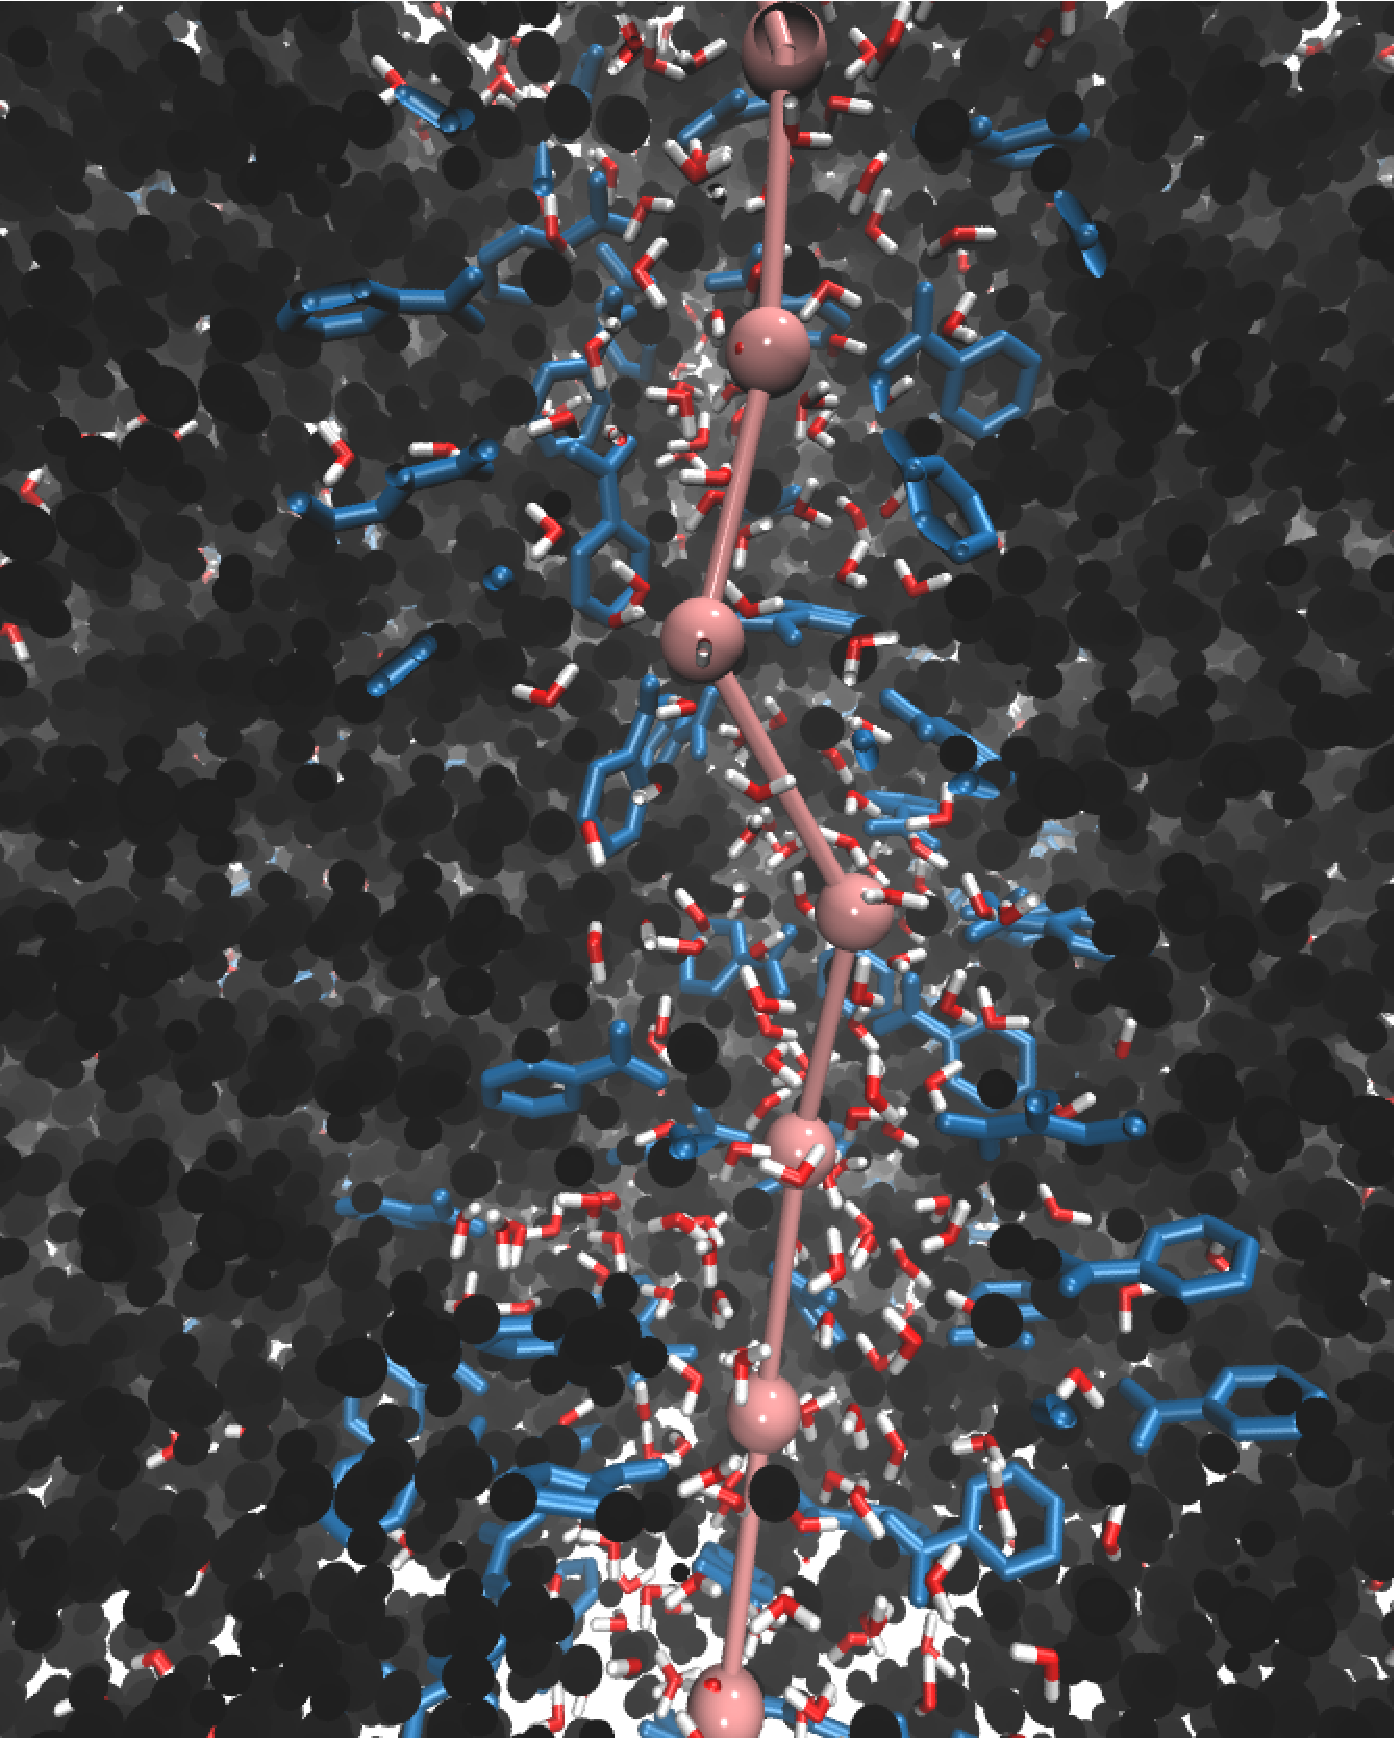
\includegraphics[width=0.45\textwidth]{spline.pdf}
  \caption{We traced the center of each pore as a function of $z$ using a spline (pink
  line). We constructed the spline in each pore using 10 points (pink spheres) whose
  positions we defined based on the center of mass of the head groups in closest proximity
  to the spline point in the $z$-direction.}\label{fig:spline}
  \end{figure}
  
  We calculated the tortuosity, $\tau$, of the pores by calculating the 
  ratio $\dfrac{L}{Z}$ where $L$ is the length of the spline and $Z$ is 
  the length of the unit cell in the $z$-direction. The average tortuosity
  of each pore is 1.03 $\pm$ 0.01 and 1.07 $\pm$ 0.02 in the 5 and 10 wt\%
  water systems respectively.
  
%  \clearpage
%  \section{Total Membrane Density}\label{section:total_density}
%  BJC: moved to main text
%  
%  In our simulations, we observe that water partitions into the tail region
%  because of the tails' low density. We plotted the density of all atoms in 
%  the system as function of their $xy$ positions within the unit cell. The 
%  pore centers of the 5 and 10 wt \% water systems have a relatively low density
%  that is comparable to the density in the tails far from the pore center
%  (see figures~\ref{fig:total_density_5wt} and~\ref{fig:total_density_10wt}).
%  The density is highest near the middle of the tails. The observed density distribution
%  is necessary in order for the wedge-shaped monomers to fill space and stay in
%  the hexagonal phase. Accordingly, water is densest in the pore center and at 
%  the tail ends (see figures~\ref{fig:total_water_density_5wt} 
%  and~\ref{fig:total_water_density_10wt}). Very little water is present in the 
%  dense mid-tail region. 
%  
%  \begin{figure}[!htb]
%  \centering
%  \begin{subfigure}{0.45\textwidth}
%  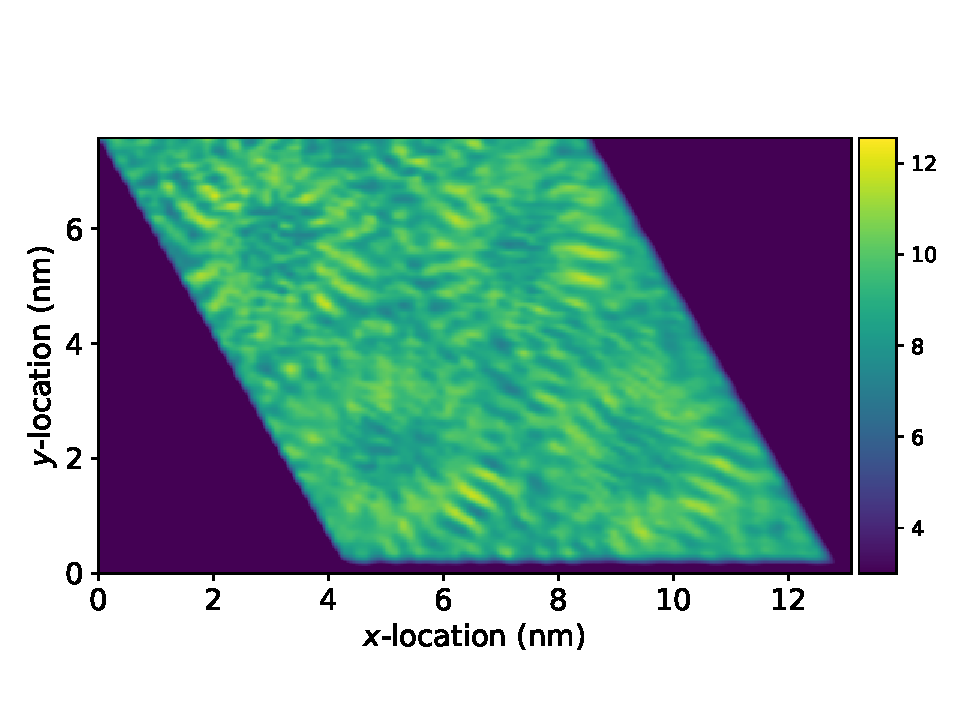
\includegraphics[width=\textwidth]{total_density_5wt.pdf}
%  \caption{5 wt \% water, spatial density of all atoms}\label{fig:total_density_5wt}
%  \end{subfigure}
%  \begin{subfigure}{0.45\textwidth}
%  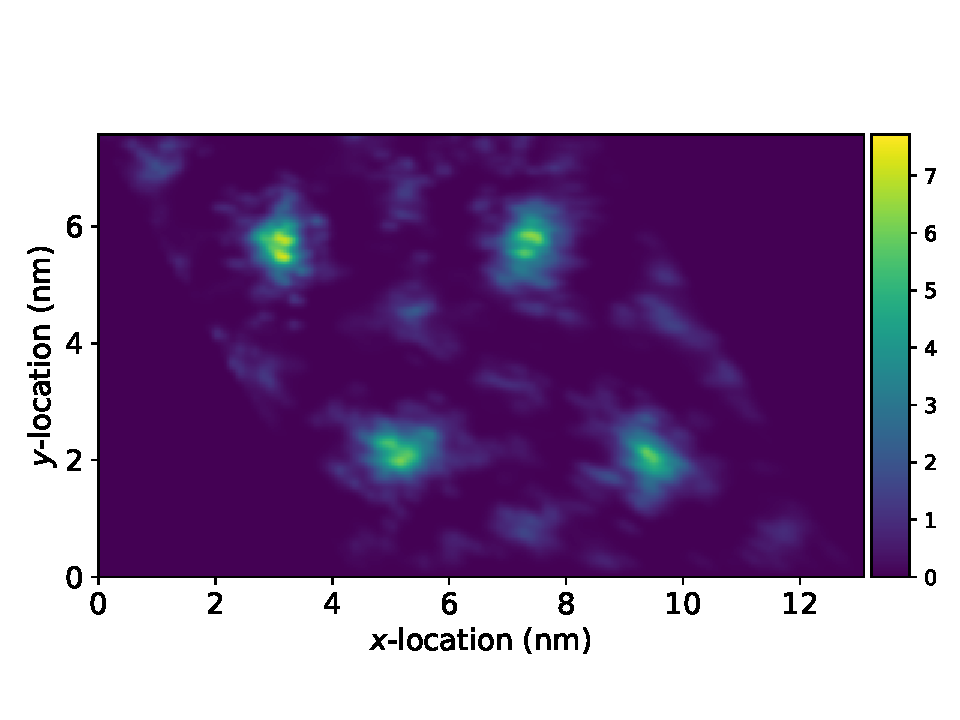
\includegraphics[width=\textwidth]{total_water_density_5wt.pdf}
%  \caption{5 wt \% water, spatial density of water}\label{fig:total_water_density_5wt}
%  \end{subfigure}
%  \begin{subfigure}{0.45\textwidth}
%  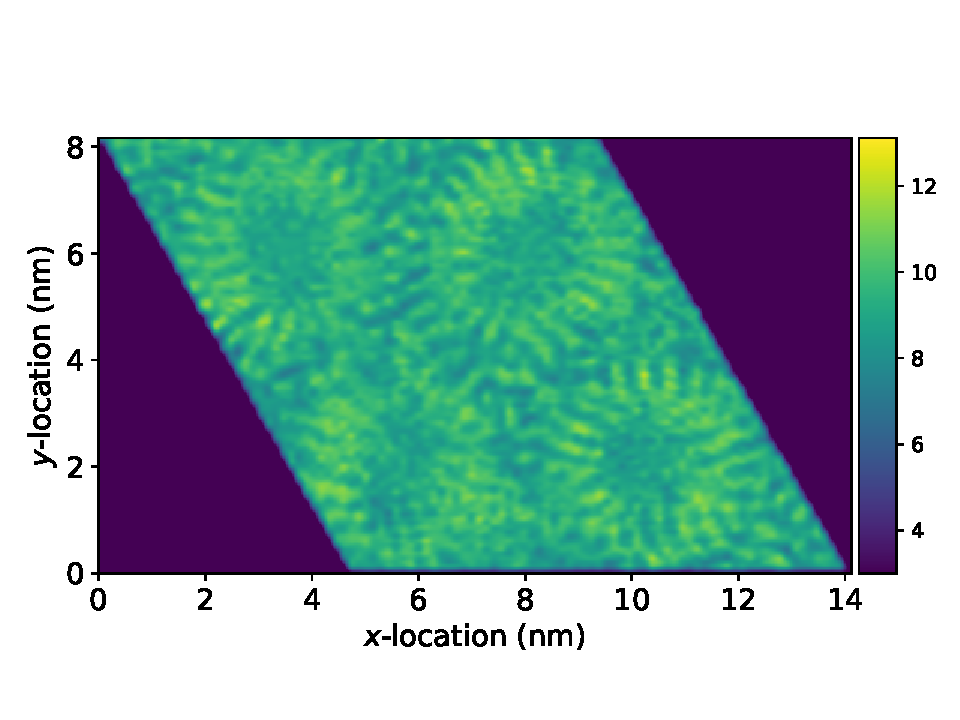
\includegraphics[width=\textwidth]{total_density_10wt.pdf}
%  \caption{10 wt \% water, spatial density of all atoms}\label{fig:total_density_10wt}
%  \end{subfigure}
%  \begin{subfigure}{0.45\textwidth}
%  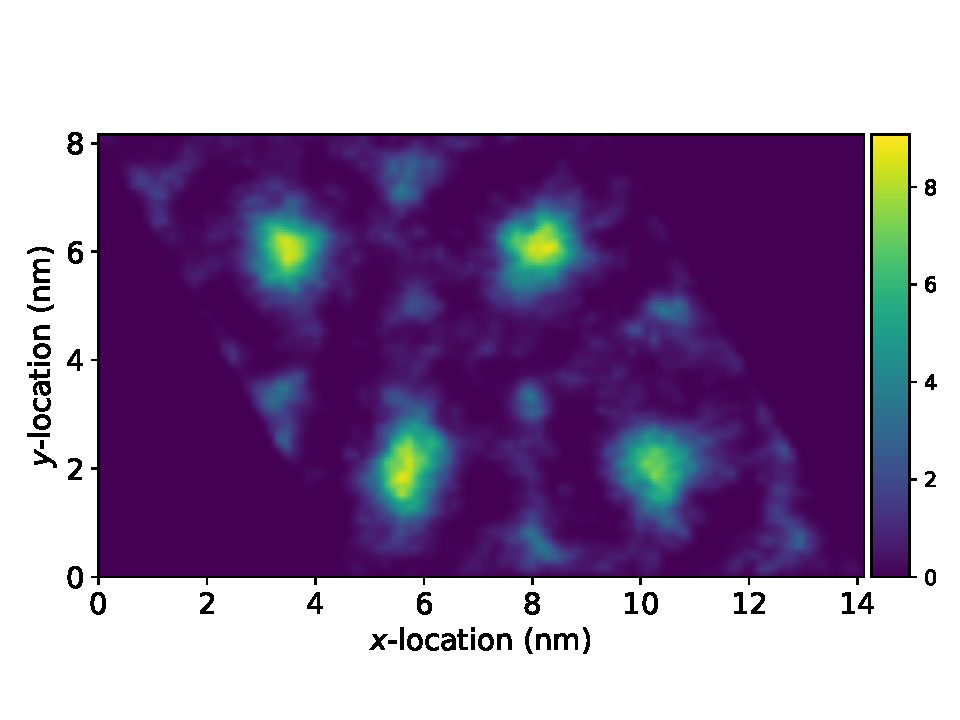
\includegraphics[width=\textwidth]{total_water_density_10wt.pdf}
%  \caption{10 wt \% water, spatial density of water}\label{fig:total_water_density_10wt}
%  \end{subfigure}
%  \caption{The lowest density regions of both membranes are in the pore center and in the
%  tail region, furthest from the pore center (a \& c). Water is densest in the low density
%  regions (b \& d).}\label{fig:total_density}
%  \end{figure}

%  \clearpage
%  \section{Solute Pairing with Sodium}
%
%  \begin{figure}[!htb]
%  \centering
%  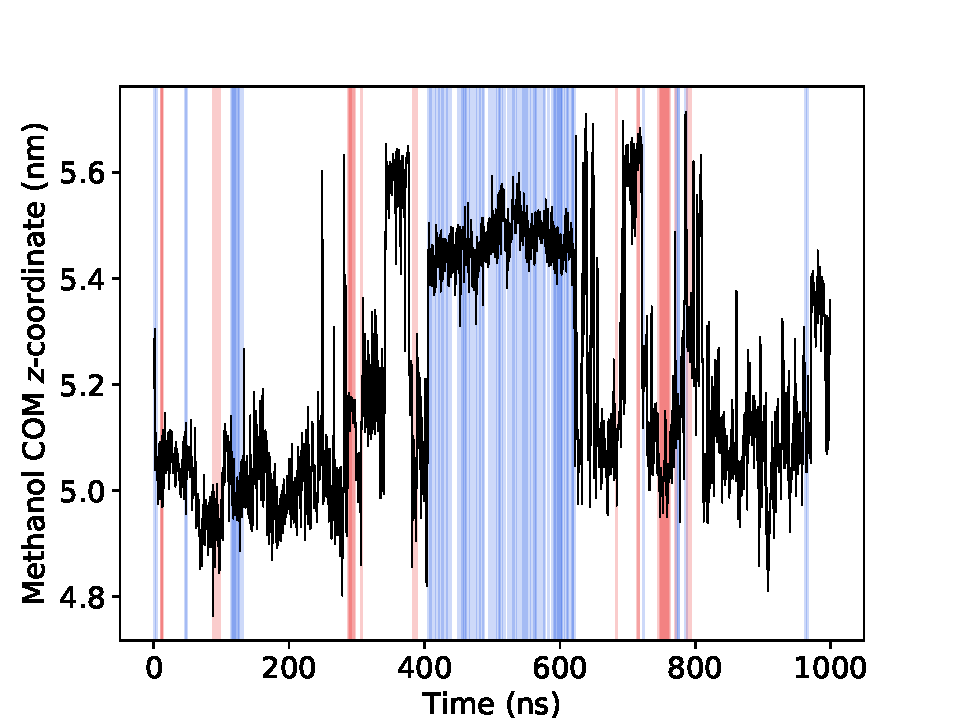
\includegraphics[width=0.45\textwidth]{na_met_trace.pdf}  % create with nn.py located in MET/10wt
%  \caption{The oxygen atom of methanol stays within 2.5 \AA~of the same sodium ion for
%  the majority of the trapping occurrence between 400 and 600 ns. Regions
%  highlighted red or blue indicate times when methanol's oxygen atom is within 
%  2.5 \AA~of a sodium ion. The color of the shaded regions are switched every time
%  the oxygen atom becomes associated to a different sodium ion.}\label{fig:na_met_trace}
%  \end{figure}
%  
%  \section{Mercaptoethanol's range of behavior}
%  
%  \begin{figure}
%  \centering
%  \begin{subfigure}{0.45\textwidth}
%  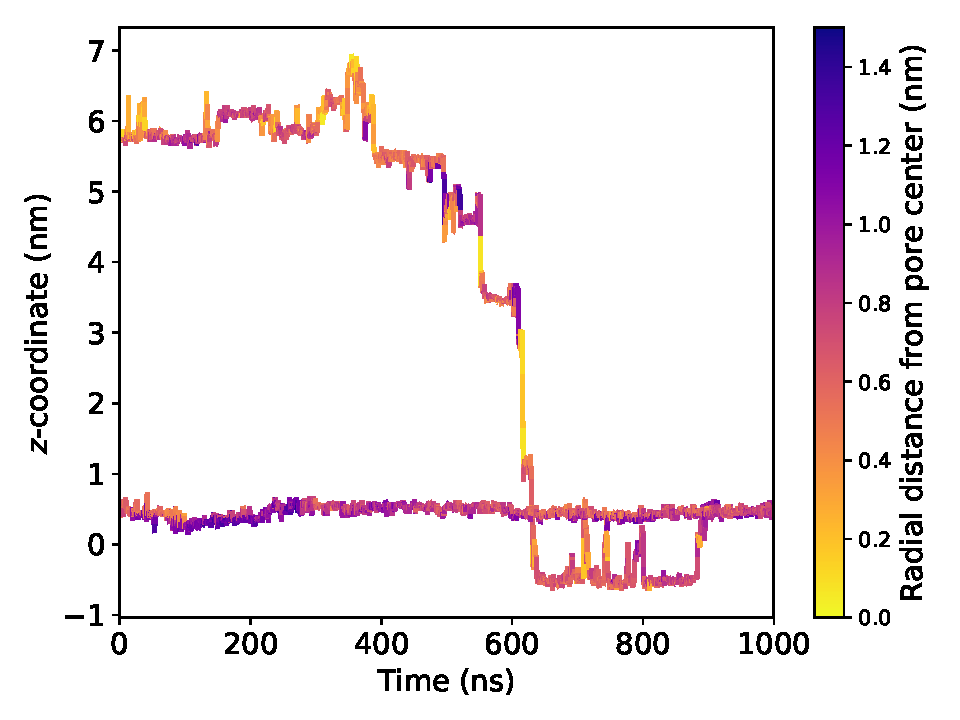
\includegraphics[width=\linewidth]{SOH_trace.pdf}
%  \caption{}\label{fig:SOH_trace}
%  \end{subfigure}
%  \caption{Mercaptoethanol exhibits transport behavior ranging from frequent hopping
%  to lengthy trapping. Large hops generally occur near the pore center while 
%  long entrapments occur while tangled among the monomer tails.}
%  \end{figure}
%  
%  \section{THF-sodium Complexation}
%  
%  \begin{figure}
%  \centering
%  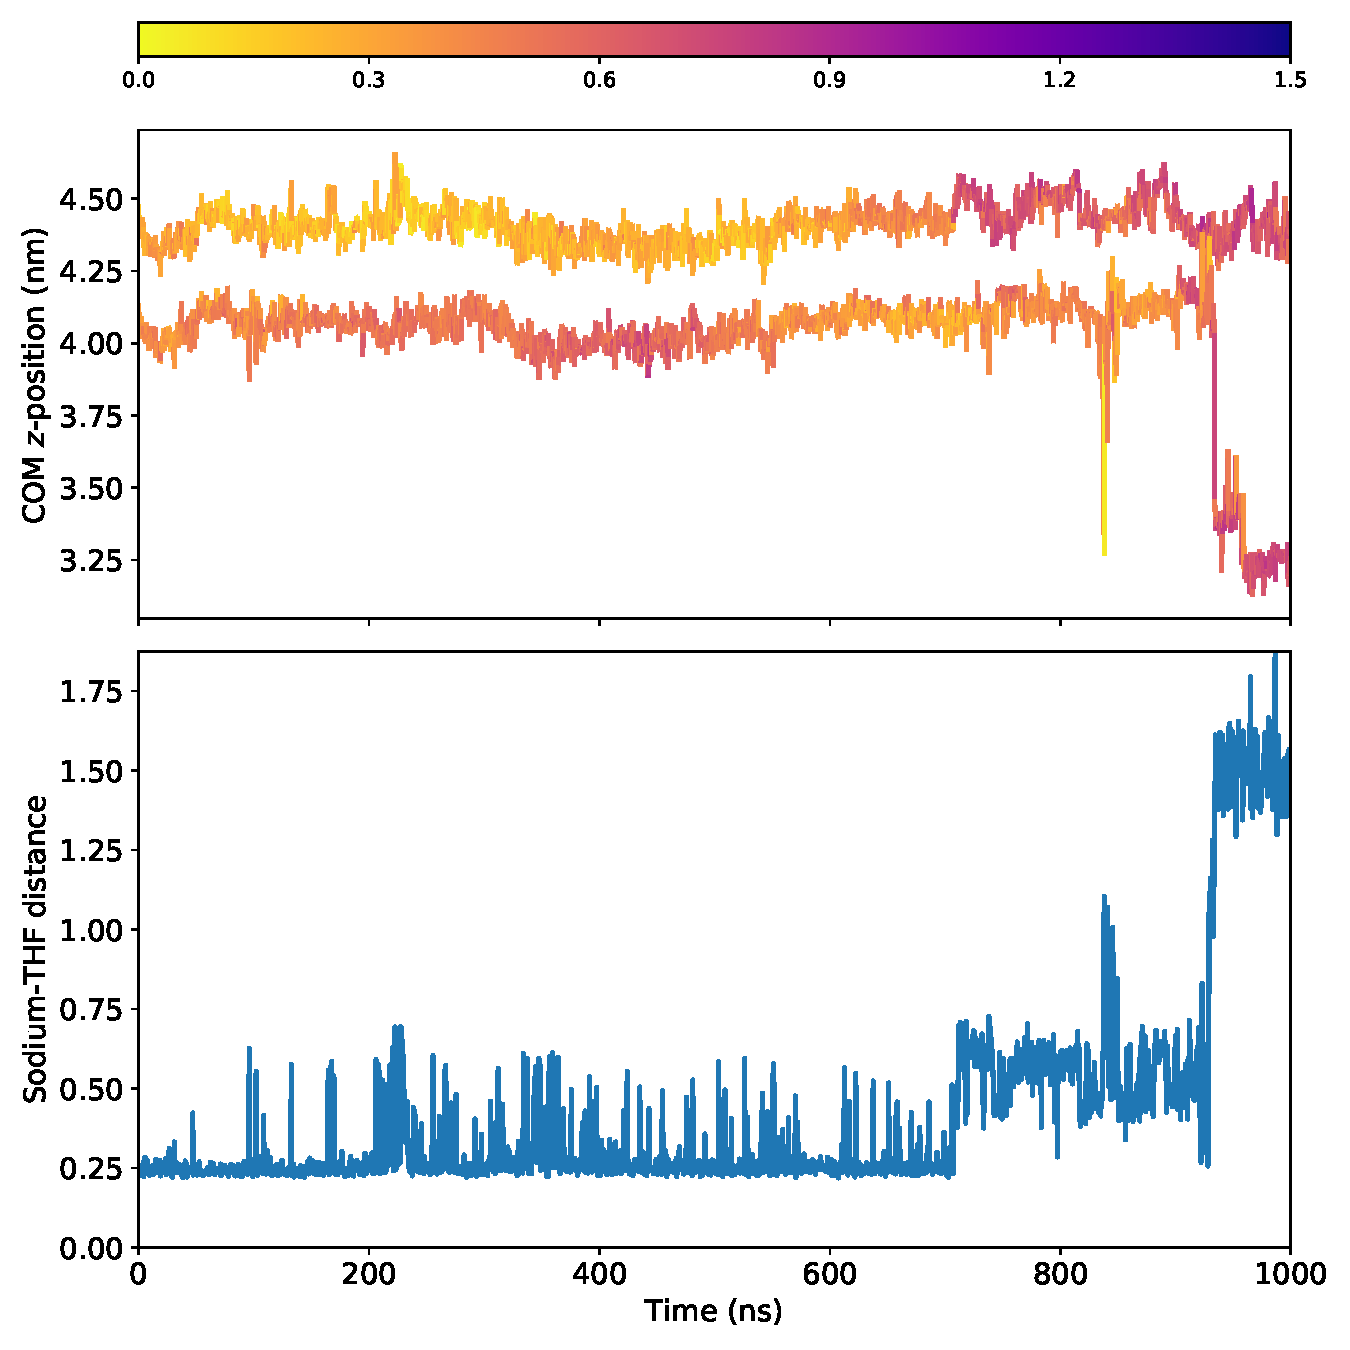
\includegraphics[width=0.5\textwidth]{thf_sodium_coordination.pdf}
%  \caption{Coordination of THF with sodium ions may help stabilize it inside the
%  pore region. For the first 700 ns of the trajectories shown, the center of mass
%  of THF (top line in top figure) and a sodium ion (bottom line in top figure) move
%  in tandem. The distance between the oxygen atom of THF and the sodium ion has only
%  occasional fluctuations away from a relatively stable separation of ca. 0.25 nm. 
%  After 700 ns, THF separates from the sodium ion and moves closer to the head group
%  region.}\label{fig:thf_sodium_coordination}
%  \end{figure}
  %MRS2: Can we show something that describes a distribution of multiple THF? this is just one, 
  % which is suggestive, but this sort of suggestive information maybe should be in supporting. 
  %MRS2: did you trace down any information on THF-ion complexation? We should be able to report on whether
  %this is physical or a force field artifact.
  % BJC2: probably better to find evidence of ether-ion complexation since it applies to multiple
  % solutes that we studied
  
% BJC: the arguments in the following section aren't as strong as I want them to be. 
% And not necessary for this paper.
%
%  \section{Choosing a transport model}\label{section:transport_model_selection}
%
%  We used the toolbox created by Meroz and Sokolov in order to justify our
%  choice of transport model.\cite{meroz_toolbox_2015} The solutes in our systems
%  exhibit anomalous transport properties characteristic of a Continuous Time
%  Random Walk (CTRW). 
%
%  \subsection*{Mean Squared Displacement}
%
%  The general form of a mean squared displacement (MSD) curve is:
%  \begin{equation}
%	\langle x^2(t) \rangle \sim t ^ \alpha
%	\label{eqn:msd}
%  \end{equation}
%  For Brownian motion, $\alpha = 1$ and the MSD is linear. When $\alpha \neq
%  1$, the particle of interest exhibits anomalous diffusion. Values of $\alpha$
%  greater than 1 give rise to superdiffusion, while values of $\alpha$ less than
%  1 give rise to subdiffusion.
%
%  We can calculate the ensemble-averaged MSD curve by averaging the MSDs of
%  each particle trajectory, where each MSD is calculated using:
%  \begin{equation}
%	\delta^2(t) = \| \mathbf{r}(t) - \mathbf{r}(0) \|^2
%	\label{eqn:ensemble_msd}
%  \end{equation}
%  where $\|\cdot\|$ represents the Euclidean norm. 
%
%  The mean squared displacement of solutes in our model is a non-linear
%  function of time, with $\alpha < 1$ which is indicative of anomalous
%  subdiffusion. Figure \ref{fig:msd_power_law}a plots the ensemble-averaged MSD
%  curve for 24 ethanol molecules diffusing in a 10 wt\% water H\textsubscript{II}
%  LLC membrane system. We fit a power law of the form $Ae^{\alpha}$ to the MSD
%  curve. We performed 2000 bootstrap trials by randomly sampling 24 MSD curves
%  with replacement from the 24 total ethanol MSD curves. The bootstrapped average
%  value of $\alpha$ is 0.75 for this system. 
% 
%  \begin{figure}[!htb]
%  \centering
%% Generated with : msd.py -t PR_nojump.xtc -g PR.gro -r ETH -ensemble -power_law -a z -nboot 2000
%% in directory: /home/bcoscia/Documents/Gromacs/Transport/NaGA3C11/ETH/10wt
%  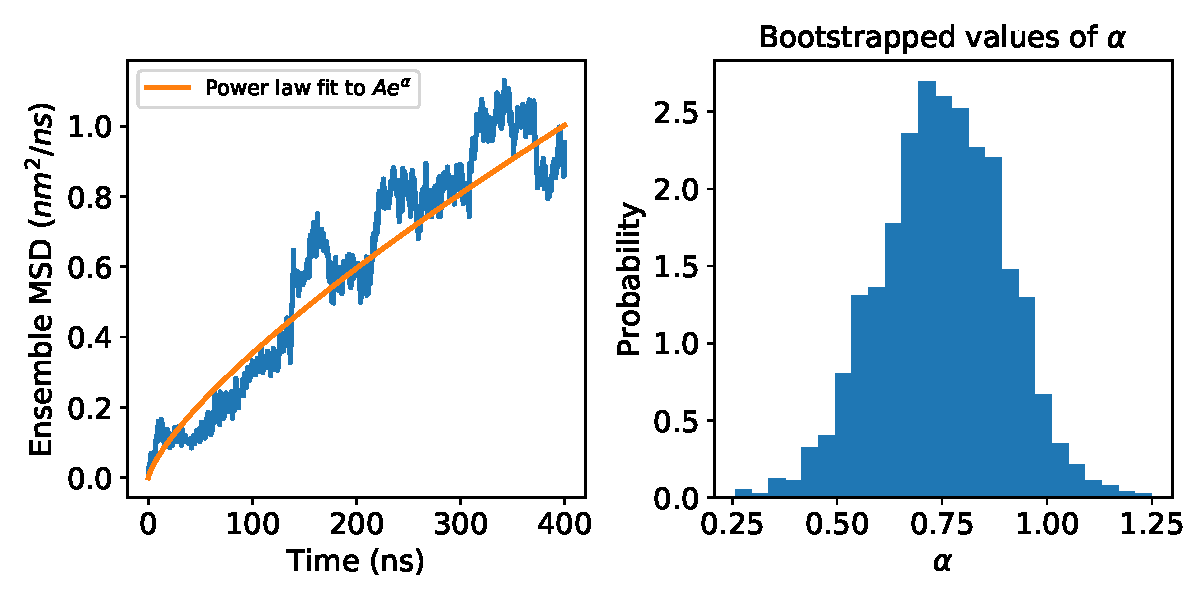
\includegraphics[width=0.8\linewidth]{msd_power_law.pdf}
%  \caption{(a) We fit a curve with the form of Equation~\ref{eqn:msd} to the
%	  ensemble-averaged MSD curve. (b) The average value of $\alpha$, obtained using
%	  fits to MSDs calculated from bootstrapped ensembles, is less than 1 suggesting
%	  that ethanol molecules in our model exhibit subdiffusive
%	  behavior.}\label{fig:msd_power_law}
%  \end{figure}
%
%  \subsection*{Ergodicity}
%
%  The ergodicity of a system can help us narrow down the possible anomalous
%  diffusion mechanisms. In an ergodic system, the time-averaged behavior of an
%  observable should yield the same result as the ensemble average of the same
%  observable. Examples of anomalous diffusion processes that are ergodic include
%  random walks on fractals (RWF) and fractional Brownian motion (FBM).
%  Non-ergodic systems generally give rise to CTRWs with the possibility of
%  combination with a RWF and/or FBM.\cite{meroz_toolbox_2015} 
%
%  We tested the ergodicity of our system by comparing the ensemble-averaged
%  and time-averaged MSD curves. We calculated the MSD of each ethanol trajectory
%  using Equation~\ref{eqn:ensemble_msd} and a time-averaged algorithm: 
%  \begin{equation}
%	\delta^2(t) = \dfrac{1}{N-t} \sum_{i=0}^{N-t-1} \| \mathbf{r}(i + t) - \mathbf{r}(i) \|^2
%  \end{equation}
%  where N is the total number of simulation frames, and t represents the length
%  of subinterval or number of frames per subinterval. We averaged the MSD curves
%  from each trajectory in order to create final MSD plots.
%
%  The ethanol molecules exhibit non-ergodic behavior because their
%  time-averaged and ensemble-averaged MSDs do not agree with each other
%  (Figure~\ref{fig:ethanol_msd_comparison}). We validated our analysis using a 1
%  ns simulation of a box of tip3p water molecules. As expected, since the
%  particles exhibit Brownian motion, the time-averaged and ensemble-averaged MSDs
%  agree with each within error (Figure~\ref{fig:water_box_msd_comparison}).
%
%  \begin{figure}[!htb]
%  \centering
%  \begin{subfigure}{0.45\textwidth}
%% Generated with : msd.py -t PR_nojump.xtc -g PR.gro -r ETH -compare -nboot 2000 -a z
%% in directory: /home/bcoscia/Documents/Gromacs/Transport/NaGA3C11/ETH/10wt
%  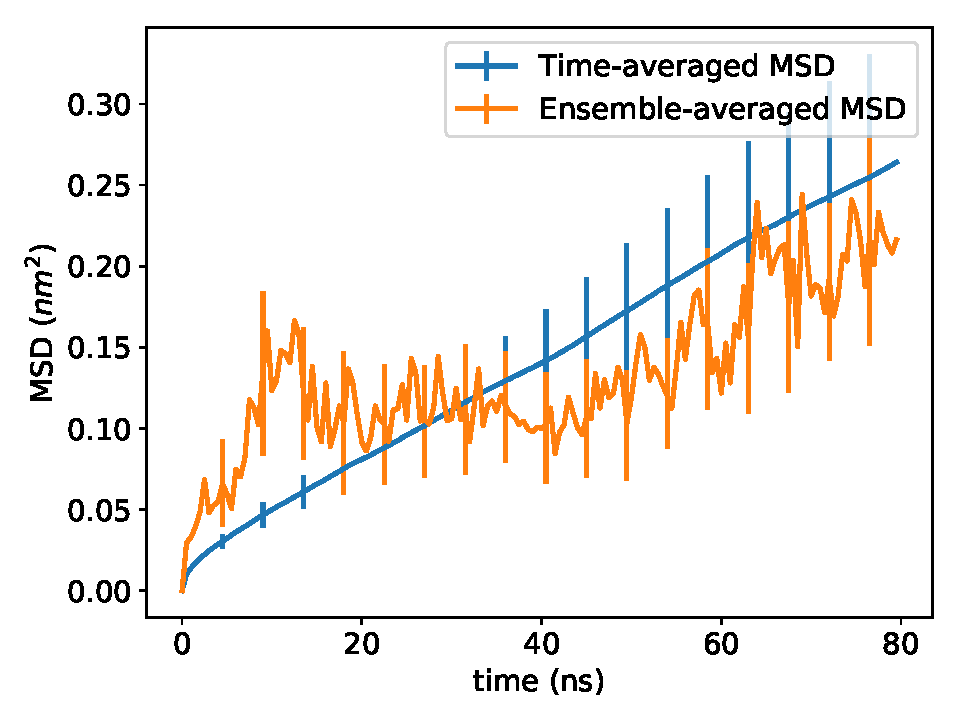
\includegraphics[width=\textwidth]{ethanol_msd_comparison.pdf}
%  \caption{}\label{fig:ethanol_msd_comparison}
%  \end{subfigure} 
%  \begin{subfigure}{0.45\textwidth}
%% Generated with msd.py -t traj_nojump.xtc -g npt.gro -r SOL -compare --fracshow 0.4 -nboot 2000 -a z
%% in directory: /home/bcoscia/Documents/Gromacs/Transport/Solvent/solvent_boxes/pure_water
%  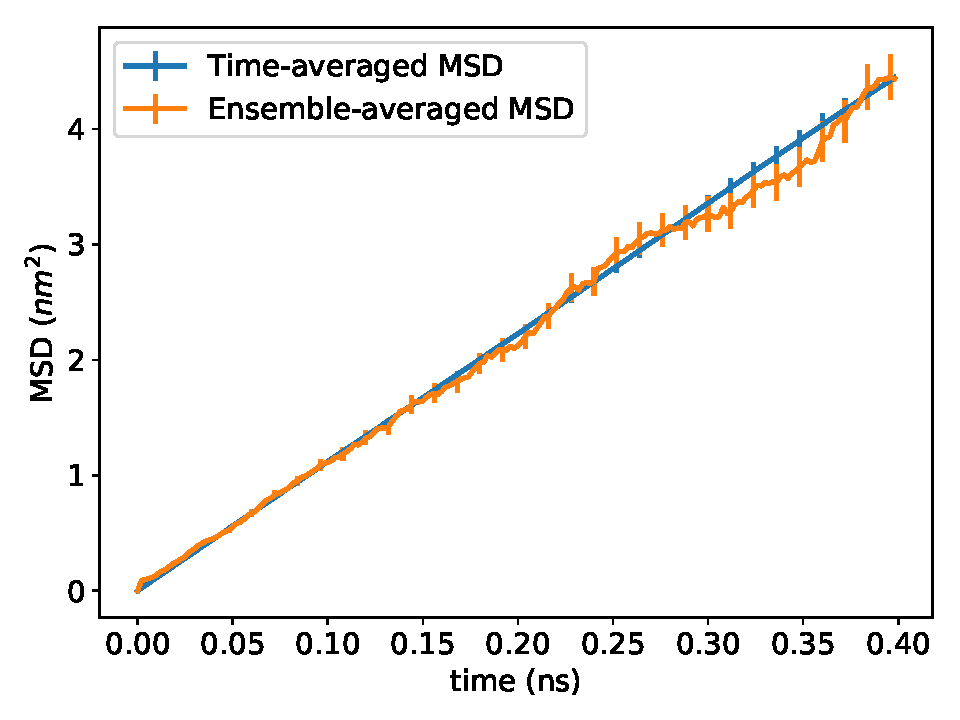
\includegraphics[width=\textwidth]{water_box_msd_comparison.pdf}
%  \caption{}\label{fig:water_box_msd_comparison}
%  \end{subfigure} 
%  \caption{(a) The time-averaged and the ensemble-averaged MSDs for ethanol in
%	  an H\textsubscript{II} nanopore are not in agreement, implying non-ergodicity.
%	  (b) A box of tip3p water molecules is expected to be ergodic and it is shown to
%	  be true here because both MSDs are in agreement. }\label{fig:msd_comparison}
%  \end{figure}
%
%  \subsection*{Autocorrelation of steps}
%
%% From Sokolov paper: "Assigning different waiting times τ i to each step, and assuming that the
%% steps are uncorrelated as in a regular RW, gives rise to the CTRW model" -- I
%% might need to check autocorrelation of steps lengths when a hop occurs rather
%% than every time step. Not sure if there is enough data for that, but could check 
%% a particularly hoppy trajectory after longer simulation.
%
%
%  Based on the previous two sections, our model can likely be studied as a CTRW. 
%  However, it is still possible that our CTRW model might also be convoluted with
%  an FBM or a RWF process. In a pure CTRW, the steps are uncorrelated. 
%  Both FBM and RWF exhibit anti-correlated steps. 
%
%  The steps in our system are not correlated. We showed this by calculating the
%  autocorrelation function (ACF) of the step lengths in the $z$-direction. The
%  ACF of a representative trajectory is shown in Figure~\ref{fig:eth_autocorrelation}.  
%  
%  \begin{figure}[!htb]
%  \centering
%% Generated with brownian_test.py -t PR_nojump.xtc -g PR.gro -r ETH (and appropriate uncommenting -- need to rework that script)
%% in directory: /home/bcoscia/Documents/Gromacs/Transport/NaGA3C11/ETH/10wt
%  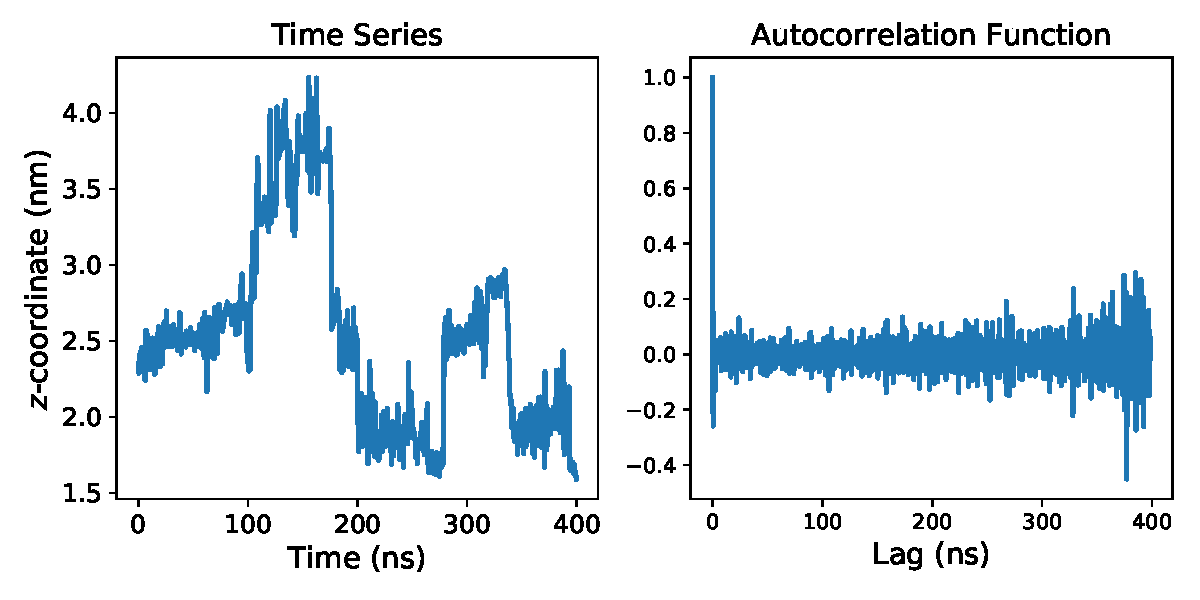
\includegraphics[width=0.8\textwidth]{eth_autocorrelation.pdf}
%  \caption{The autocorrelation function (right) of a representative ethanol
%	   center of mass $z$-coordinate trajectory (left) almost immediately decays to zero,
%	   indicating a complete loss of memory of it's previous position. Noise increases
%	   at large time lags due to decreased sampling.}\label{fig:eth_autocorrelation}
%  \end{figure}

%  \clearpage
%  \bibliography{transport}

\end{document}

% LocalWords:  LLC solutes py solvated GROMACS mdp solute ctrw GitHub equil xtc
% LocalWords:  kinetically gro gmx solvate der Waals wt PR savename pl pr trr
% LocalWords:  plateaued xlinked BJC MSDs Gierer Wirtz MSD SE tamsds hbond dist
% LocalWords:  tetrose ribose glcyol png tortuosity nn methanol's THF ca Meroz
% LocalWords:  Mercaptoethanol's Mercaptoethanol Complexation complexation msd
% LocalWords:  Sokolov superdiffusion subdiffusion nojump ETH nboot RWF FBM npt
% LocalWords:  subdiffusive CTRWs traj fracshow nanopore RW hoppy ACF brownian
